\documentclass[]{article}\usepackage[]{graphicx}\usepackage[]{color}
%% maxwidth is the original width if it is less than linewidth
%% otherwise use linewidth (to make sure the graphics do not exceed the margin)
\makeatletter
\def\maxwidth{ %
  \ifdim\Gin@nat@width>\linewidth
    \linewidth
  \else
    \Gin@nat@width
  \fi
}
\makeatother

\definecolor{fgcolor}{rgb}{0.345, 0.345, 0.345}
\newcommand{\hlnum}[1]{\textcolor[rgb]{0.686,0.059,0.569}{#1}}%
\newcommand{\hlstr}[1]{\textcolor[rgb]{0.192,0.494,0.8}{#1}}%
\newcommand{\hlcom}[1]{\textcolor[rgb]{0.678,0.584,0.686}{\textit{#1}}}%
\newcommand{\hlopt}[1]{\textcolor[rgb]{0,0,0}{#1}}%
\newcommand{\hlstd}[1]{\textcolor[rgb]{0.345,0.345,0.345}{#1}}%
\newcommand{\hlkwa}[1]{\textcolor[rgb]{0.161,0.373,0.58}{\textbf{#1}}}%
\newcommand{\hlkwb}[1]{\textcolor[rgb]{0.69,0.353,0.396}{#1}}%
\newcommand{\hlkwc}[1]{\textcolor[rgb]{0.333,0.667,0.333}{#1}}%
\newcommand{\hlkwd}[1]{\textcolor[rgb]{0.737,0.353,0.396}{\textbf{#1}}}%
\let\hlipl\hlkwb

\usepackage{framed}
\makeatletter
\newenvironment{kframe}{%
 \def\at@end@of@kframe{}%
 \ifinner\ifhmode%
  \def\at@end@of@kframe{\end{minipage}}%
  \begin{minipage}{\columnwidth}%
 \fi\fi%
 \def\FrameCommand##1{\hskip\@totalleftmargin \hskip-\fboxsep
 \colorbox{shadecolor}{##1}\hskip-\fboxsep
     % There is no \\@totalrightmargin, so:
     \hskip-\linewidth \hskip-\@totalleftmargin \hskip\columnwidth}%
 \MakeFramed {\advance\hsize-\width
   \@totalleftmargin\z@ \linewidth\hsize
   \@setminipage}}%
 {\par\unskip\endMakeFramed%
 \at@end@of@kframe}
\makeatother

\definecolor{shadecolor}{rgb}{.97, .97, .97}
\definecolor{messagecolor}{rgb}{0, 0, 0}
\definecolor{warningcolor}{rgb}{1, 0, 1}
\definecolor{errorcolor}{rgb}{1, 0, 0}
\newenvironment{knitrout}{}{} % an empty environment to be redefined in TeX

\usepackage{alltt}

%\VignetteIndexEntry{Maximized Monte Carlo: an R package}
%\VignetteEngine{knitr::knitr}
%\VignetteEncoding{UTF-8}

\usepackage{graphicx, float, amssymb, amsmath, titlesec}
\usepackage[citestyle=authoryear, natbib=true, backend=bibtex]{biblatex}
\bibliography{MaxMC-package-biblio}


\addcontentsline{toc}{section}{References}

%Code for subsubsubsection
\setcounter{secnumdepth}{4}
\titleformat{\paragraph}
{\normalfont\normalsize\bfseries}{\theparagraph}{1em}{}
\titlespacing*{\paragraph}
{0pt}{3.25ex plus 1ex minus .2ex}{1.5ex plus .2ex}

\newcommand{\pkg}[1]{{\normalfont\fontseries{b}\selectfont #1}}
\let\proglang=\textsf
\let\code=\texttt

\DeclareMathOperator{\Corr}{Corr}
\DeclareMathOperator{\Var}{Var}
\DeclareMathOperator{\Cov}{Cov}
\DeclareMathOperator{\E}{\mathbb{E}}
\DeclareMathOperator{\R}{\mathbb{R}}
\DeclareMathOperator{\dist}{\mathcal{F}}



\IfFileExists{upquote.sty}{\usepackage{upquote}}{}
\begin{document}

\title{Maximized Monte Carlo: an \proglang{R} package}
\author{Julien Neves \thanks{Graduate student, Department of Economics, Cornell University}}
\date{July 10th, 2018}

\maketitle

\begin{abstract}
	This paper describes the \proglang{R} package \pkg{MaxMC}, which implements the Maximized Monte Carlo (MMC) technique and the simple Monte Carlo technique with tie-breaker for discrete statistics. To illustrate how to use the \pkg{MaxMC} package, we present two examples: a goodness-of-fit test and the Behrens-Fisher problem.

	We perform a simulation study, in order to demonstrate the utility of the package, of irregular Wald-type tests and unit root tests for autoregressive models. We compare the MMC procedure implemented in the \pkg{MaxMC} package to the parametric bootstrap and usual asymptotic tests in both cases.
\end{abstract}

\clearpage

\tableofcontents

\clearpage

\section{Introduction}
\label{intro}

In the past several years, Monte Carlo methods have become progressively more popular. Nowadays, most statistical software will offer some sort of simulation-based techniques for data analysis (e.g. parametric bootstrap, Markov Chain Monte Carlo (MCMC) algorithm, Evolutionary Monte Carlo (EMC) algorithm, etc.). A quick search on the Comprehensive \proglang{R} Archive Network (CRAN) reveals that already many packages implement some Monte Carlo techniques; see \pkg{boot} \citep{canty_boot:_2016}, \pkg{mcmc} \citep{geyer_mcmc:_2015}, \pkg{MCMCpack} \citep{martin_mcmcpack:_2011}, \pkg{PAWL} \citep{bornn_pawl:_2012}, \pkg{ggmcmc} \citep{fernandez-i-marin_ggmcmc:_2016}, \pkg{exactLoglinTest} \citep{caffo_exactloglintest:_2013}.

Monte Carlo techniques were first introduced independently by \cite{dwass_modified_1957} and by \cite{barnard_comment_1963}; for a review, see \cite{dufour_monte_2003}. The method they proposed details a simple procedure to implement exact tests based on pivotal statistics (i.e. when the distribution does not depend on any nuisance parameters). As a matter of fact, the method only requires that the statistic can be simulated, it does not impose tractability to the distribution of statistic.

The Monte Carlo technique is akin to the parametric bootstrap in that both methods rely on simulating a fully parametric model under the null in order to make any inference. The difference lies in that the parametric bootstrap is only asymptotically justified while the Monte Carlo technique p-value corrects for finite-sample distributions.

Note that the original Monte Carlo technique, as described by \cite{dwass_modified_1957} and \cite{barnard_comment_1963}, is only valid for statistics with continuous distributions. The problem that arises is due to the possible presence of ties in the simulated values for statistics with discrete distributions. \cite{dufour_monte_2006} provides an extension of the method to circumvent this problem known as the Monte Carlo with tie-breaker technique (MC with tie-breaker).

Even though the Monte Carlo technique provides a straightforward procedure to build exact tests, one of its main shortfalls is the requirement that the finite-sample distribution of the statistic be free of any nuisance parameters. Sadly, statistics of interest in economics usually depend on some nuisance parameters. Techniques such as the bootstrap and its variants provide asymptotically valid method of inference when the distribution of the statistic is not stable. In order to retrieve exactness in tests where the finite-sample distribution of the statistic depends on some nuisance parameters, \cite{dufour_monte_2006} proposed an extension of the original Monte Carlo technique to deal with such complications also known as the Maximized Monte Carlo (MMC).

In this paper, we present an implementation of both the MMC and MC with tie-breaker techniques as described by \cite{dufour_monte_2006} for \proglang{R} through the \pkg{MaxMC} package. Readers should note that the main goal of the \pkg{MaxMC} package is not to replace any existing package, but to supplement \proglang{R} users with an accessible and effortless way to apply Monte Carlo tests, and more specifically the MMC procedure which is not yet available anywhere. In order to demonstrate where the use of the \pkg{MaxMC} package could be advantageous, we investigate two different types of common tests: Wald-type tests and unit root tests.

First, we look at Wald-type tests. The popularity of Wald-type tests can be attributed to the fact that they offer a simple way of testing a wide array of linear and non-linear restrictions using only estimators of the unrestricted model. One issue Wald-type statistics is that, since they are based on asymptotically normal estimators, they need strong regularity assumptions in order to derive any valid inference. Under these regularity conditions, the usual Wald statistic is asymptotically distributed as a chi-squared with degrees of freedom equal to the number of restrictions. As described by \cite{dufour_wald_2013}, these regularity conditions will be violated whenever the covariance matrix of the set of restrictions does not have full column rank in an open neighborhood of the true value of the parameter vector. Note that this does not preclude the  covariance matrix of the set of restrictions to have full column rank in finite samples. Indeed, we could have a covariance matrix where in finite sample the matrix is well-defined and invertible, but, as the sample size goes to infinity, the covariance matrix would converge to a singular matrix. Then, in this case, regularity conditions would be violated. As a matter of fact, situations of this type might be more common than one would first assume. \cite{dufour_wald_2013} list a set of common examples where regularity conditions needed by the Wald-type statistics are breached due to an asymptotically singular covariance matrix of the set of restrictions, including, but not limited to, tests of Granger non-causality in VARMA models, see \cite{boudjellaba_testing_1992, boudjellaba_simplified_1992}, and test of volatility and co-volatility, see \cite{gourieroux_size_2013}.

Note that, as stated previously, the Wald statistic can be well-defined in finite sample while converging to a singular matrix as the sample size goes to infinity. Accordingly, Monte Carlo techniques will yield valid inference as they do not rely on the existence of the asymptotic distribution of the statistic, but simply require that we can simulate the finite-sample distribution. As such, Monte Carlo techniques should be robust to this type of violation of regularity conditions, and will allow us to use Wald-type tests even in situations where the usual asymptomatic critical values are invalid or at best misleading.

Second, we turn our attention to test for the order of integration of time series. Since multiple time-series in economics can be characterized as integrated processes of different order, the problem of testing for the presence of integration has been study extensively in the past decades. One of the most important tests for the presence of unit roots in time-series comes from \cite{dickey_distribution_1979,fuller_introduction_1976}. Their test based on random walk processes was later extended to processes of order $p$, also known as augmented Dickey-Fuller tests.


Now, the augmented Dickey-Fuller type tests are based on I(1) processes and do not technically preclude I(2) processes. But, as described in \cite{david_a._dickey_determining_1987}, \cite{haldrup_robustness_2002} and \cite{pantula_testing_1989}, the null-distribution of the augmented Dickey-Fuller statistic is not invariant to the order of integration of the process. In fact, \cite{david_a._dickey_determining_1987} showed using Monte Carlo simulations that when testing for a unit root in an I(2) process, the lower-tailed test critical values given in \cite[Table 8.5.2]{fuller_introduction_1976} will slightly over-reject. Additionally,  \cite{haldrup_robustness_2002} confirmed that the lower-tail of the distribution (associated with $H_1: \gamma<0$) is only slightly affected by the presence of a unit root of multiplicity of 2, but, \cite{haldrup_robustness_2002} also showed that the upper-tail of the distribution (associated with $H_1: \gamma>0$) is severely distorted. Therefore, in this paper we present a way to correct for this distortion using the MMC technique developed by \cite{dufour_monte_2006} and implemented in this package.

This paper is organized as follows. Section 2 provides the framework for both the MC technique with tie-breaker in the case of a discrete statistic and the MMC. Section 3 gives the details for the implementation of the \pkg{MaxMC} package. Also included in section 3 is an example of test of goodness of fit and an example based on testing the equality of means in populations with different variances to demonstrate how the \pkg{MaxMC} package can be directly applied. Section 4 sets the framework for Wald-type tests, describes four example of irregular Wald statistics, and reports their respective simulation study results. Section 5 provides the framework for the augmented Dickey-Fuller test, and the results for the unit root test simulation study. Finally, the source code of the package is provided in the appendix. Note that \textbf{.Rd} files are excluded as we are using the package \pkg{roxygen2} \citep{wickham_roxygen2:_2015} to generate them directly from our \textbf{.R} files.

\section{Monte Carlo tests}

Let $S$ be a statistic that can be simulated. Then the distribution of $S$ follows either one of the two following cases
\begin{align}
S & \sim \dist(y) \\
S & \sim \dist(y \mid \nu)
\end{align}
i.e. where the finite-sample distribution of the statistic $S$ is either pivotal or non-pivotal (i.e. dependent on some the nuisance parameter $\nu$).

\subsection{Monte Carlo with tie-breaker}

Let $H_0$ be the null hypothesis we wish to test. Then, we first look at the case where the statistic is pivotal under $H_0$ (i.e. $S \sim \dist(y)$ under $H_0$).

The usual first step for the Monte Carlo technique is to compute the statistic $S_0$ using the sample data, and then generate $\mathrm{N}$ $i.i.d$. replications $S_{j}$ for $j=1,..., N$ of $S$ under $H_0$. We do not concern ourselves for the moment with how the $S_j$ are generated, but simply assume that we are indeed able to generate them.

In order to test for $H_0$, \cite{dufour_monte_2003} provide the following p-value function
\begin{align}
\hat{p}_{N}(S_{0}) & =\frac{N\hat{G}_{n}(S_{0})+1}{N+1}
\end{align}
where $\hat{G}_{N}(x)$ is the survival function defined as
\begin{align}
	\label{eq:G_N}
	\hat{G}_{N}(x) & =\frac{1}{N}\sum_{j=1}^{N}I_{[0,\infty]}(S_{j}-x) \quad \mathrm{where} \ I_{A}(z)=\left\{\begin{array}{l}
		1\ \mathrm{if}\ z\in A\\
		0\ \mathrm{if}\ z\not\in A
	\end{array}\right.
\end{align}

Let $\alpha$ be the desired level for the test. Then, as detailed in \cite{dufour_monte_2003}, if $\alpha(N+1)$ is an integer, we have
\begin{align}
P_{H_{0}}[\hat{p}_{N}(S_{0}) & \leq\alpha]=\alpha
\end{align}
which simply implies that the following critical region
\begin{align}
	\label{eq:crit}
	\hat{p}_{N}(S_{0}) & \leq\alpha
\end{align}
has exact level equal to $\alpha$.

It is important to note that $N\hat{G}_{N}(x)$ can be equivalently described as the number of simulated values of $S$ bigger than $x$. Therefore, as described in \cite{dufour_monte_2003}, we have the following relationship
\begin{align}
\hat{G}_{n}(S_{0}) &= \frac{N+1-\hat{R}_N(S_0)}{N}
\end{align}
where $\hat{R}_N(S_0)$ represents the sample rank of $S_0$ in $S_0,S_{1},...,S_{N}$.

We can accordingly replace the following condition
\begin{align}
\hat{p}_{N}(S_{0}) & = \frac{N\hat{G}_{n}(S_{0})+1}{N+1} \leq\ \alpha
\end{align}
by
\begin{align}
\hat{p}_{N}(S_{0}) & = \frac{N + 2 -\hat{R}_N(S_0)}{N+1} \leq\ \alpha
\end{align}

As one might notice, if the test statistic is discrete, presence of ties in the sample ranks will lead to some difficulty in computing the associated p-value. Accordingly, \cite{dufour_monte_2006} provides a way of ``breaking'' the ties using the uniform distribution.

Let $U_0, U_1,...,U_N \overset{i.i.d}{\sim} U(0,1)$, then for every $S_i$, we can create a pair $(S_i,U_i)$. Using the following lexicographic preference relation
\begin{align}
(S_i,U_i) \preccurlyeq (S_0,U_0) \Longleftrightarrow \{ S_i<S_0 \ \mathrm{or} \ ( S_i = S_0 \ \mathrm{and} \ U_i \leq U_0 ) \}
\end{align}
we can order the $(S_i,U_i)$ pairs and define the randomized rank for $S_0$ as
\begin{align}
\tilde{R}_{N}(S_0) & = \sum_{i=0}^{N}I[(S_i,U_i) \preccurlyeq (S_0,U_0)]
\end{align}
where $I$ is an indicator function for the preference relation.

Therefore, the p-value is now defined as
\begin{align}
\tilde{p}_{N}(S_{0}) & = \frac{N + 2 -\tilde{R}_N(S_0)}{N+1}
\end{align}
and the test is still exact if $\alpha(N+1)$ is an integer, i.e.
\begin{align}
P_{H_{0}}[\tilde{p}_{N}(S_{0}) & \leq\alpha]=\alpha
\end{align}
for a detailed proof; see \citet{dufour_monte_2006}.

We can summarize the procedure as the following
\begin{itemize}
\item[Step 1] Compute the statistic $S_0$ using the sample data
\item[Step 2] Generate N $i.i.d.$ replications $S_{j}$ of the statistic $S$ under $H_0$
\item[Step 3] Using the replications $S_{j}$, compute the following p-value
\begin{align}
\tilde{p}_{N}(S_{0}) & = \frac{N + 2 -\tilde{R}_N(S_0)}{N+1}
\end{align}
where $\tilde{R}_N(S_0)$ is the randomized sample rank of $S_0$
\item[Step 4]  Test if $\tilde{p}_{N}(S_{0})\leq \alpha$
\end{itemize}
This procedure is known as the MC with tie-breaker, and if the statistic is pivotal and $\alpha(N+1)$ is an integer, the test is exact. Note that the distribution of the statistic is no longer required to be continuous. The MC with tie-breaker is implemented in the \pkg{MaxMC} package under the function name \code{mc}.

\subsection{Maximized Monte Carlo}

We now turn our attention to the more interesting case; when the statistic $S$ depends on some nuisance parameter $\nu$.

Let $\nu_0$ be the true value of the nuisance parameter of $S$. Then, we wish to test
\begin{align}
H_0 : & \nu_0 \in \Omega_0
\end{align}
where $\Omega_0$ is the subset of parameter space $\Omega$ consistent with the null hypothesis. To solve this type of problem and retrieve an exact procedure, \citet{dufour_monte_2006} proposed to modify the previous Monte Carlo technique as follows
\begin{itemize}
\item[Step 1] Compute the statistic $S_0$ using the sample data
\item[Step 2]  Generate N $i.i.d.$ replications $S_{j}(\nu)$ of the statistic $S$ for each $\nu \in \Omega_0$
\item[Step 3]  Using the replications $S_{j}(\nu)$, compute the following p-value
\begin{align}
\hat{p}_{N}(S_{0} \mid \nu) & = \frac{N\hat{G}_{N}(S_{0} \mid \nu)+1}{N+1}
\end{align}
where $\hat{G}_{N}(x \mid \nu$ corresponds to the following survival function
\begin{align}
\hat{G}_{N}(x \mid \nu) & =\frac{1}{N}\sum_{j=1}^{N}I_{[0,\infty]}(S_{j}(\nu)-x) \quad \mathrm{where} \ I_{A}(z)=\left\{\begin{array}{l}
1\ \mathrm{if}\ z\in A\\
0\ \mathrm{if}\ z\not\in A
\end{array}\right.
\end{align}

\item[Step 4] Maximize the p-value function $\hat{p}_{N}(S_{0} \mid \nu)$ over the set $\nu \in \Omega_0$ i.e.
\begin{align}
\hat{Q}_N(S_0) & = \sup_{\nu \in \Omega_0} \hat{p}_{N}(S_{0} \mid \nu)
\end{align}

\item[Step 5] Test if
\begin{align}
\hat{Q}_{N}(S_{0})\leq \alpha
\end{align}
\end{itemize}

If $\alpha(N+1)$ is an integer and the distribution of $S$ is continuous, then under $H_0$ we have
\begin{align}
P [\hat{Q}_n(S_0) \leq \alpha] = \alpha
\end{align}
which implies that the MMC procedure has exact level $\alpha$ for the following critical region
\begin{align}
	\hat{Q}_n(S_0) \leq \alpha
\end{align}
for a detailed proof; see \cite{dufour_monte_2006}.

This procedure is defined as the Maximized Monte Carlo (MMC) test and $\hat{Q}_n(S_0)$ as the MMC p-value.

Note that without relying on strong regularity assumptions, the MMC provides a simple method to obtain tests with valid inference even in the presence of nuisance parameters.

As for the MC with tie-breaker, it important to note that we can use ranks instead of directly using the survival function $\hat{G}_{n}(S_{0} \mid \nu)$. Therefore, as previously shown, we can write $\hat{G}_{n}(S_{0} \mid \nu)$ as
\begin{align}
\hat{G}_{n}(S_{0} \mid \nu) &= \frac{N+1-\hat{R}_N(S_0 \mid \nu)}{N}
\end{align}
where $\hat{R}_N(S_0 \mid \nu)$ represents the sample rank of $S_0$ in $S_0, S_1(\nu),...,S_N(\nu)$.

In the case of a discrete statistic, we can extend the discussion in the previous section to how to ``break'' ties in sample ranks. Hence, let $U_0, U_1,...,U_N \overset{i.i.d}{\sim} U(0,1)$, then we can create the pairs $(S_i,U_i)$ and use the following lexicographic preference relation
\begin{align}
 	(S_i(\nu),U_i) \preccurlyeq (S_0,U_0) \Longleftrightarrow \{ S_i(\nu)<S_0 \ \mathrm{or} \ ( S_i(\nu) = S_0 \ \mathrm{and} \ U_i \leq U_0 ) \}
\end{align}
 to order the $(S_i,U_i)$ pairs and compute the randomized rank for $S_0$ as
 \begin{align}
 	\tilde{R}_{N}(S_0\mid \nu) & = \sum_{i=0}^{N}I[(S_i(\nu),U_i) \preccurlyeq (S_0,U_0)]
 \end{align}
 where $I$ is an indicator function for the preference relation.

Thus, if we have that $\alpha(N+1)$ is an integer and that we can simulate $S$ then for
\begin{align}
\hat{p}_{N}(S_{0} \mid \nu) & = \frac{N + 2 -\hat{R}_N(S_0 \mid \nu)}{N+1}
\end{align}
we have that
\begin{align}
P [\sup_{\nu \in \Omega_0} \tilde{p}_{N}(S_{0} \mid \nu) \leq \alpha] = \alpha
\end{align}
which implies that the test is exact at level $\alpha$; again for a proof, see \cite{dufour_monte_2006}.

One issue that arises with the MMC is that, as the size of $\Omega_0$ increases, the method becomes computationally heavier. Thankfully, in the past decades, great improvements have been made to both computer hardware and global optimization algorithms. In fact, section 4 presents some of the global optimization algorithms that have been implemented in the \pkg{MaxMC} package in order to find the supremum of the p-value function. We can hope that future advances in computer science will render the MMC procedure an even more attractive option for any simulation-based test.

Regardless of any past or future improvments in the field of computer science, we can simplify the MMC procedure whenever a consistent point set estimate of $\nu$ is available and still maintain the validity of the inference of the test asymptotically. We simply reformulate the previous steps in the following way
\begin{itemize}
	\item[Step 1] Compute the statistic $S_0$ using the sample data
	\item[Step 2] Let $C_T$ be a sequence of sets such that $C_T \subset \Omega$, and
	\begin{align}
	\label{eq:consistent}
	\lim\limits_{T \rightarrow \infty}P[\nu_0 \in C_T] = 1 \textnormal{ under } H_0
	\end{align}
	\item[Step 3] Generate N $i.i.d.$ replications $S_{Tj}(\nu)$ of the statistic $S$ for each $\nu \in C_T$
	\item[Step 4] Using the replications $S_{Tj}(\nu)$, compute the following p-value
	\begin{align}
	\hat{p}_{N}(S_{0} \mid \nu) & = \frac{N\hat{G}_{TN}(S_{0} \mid \nu)+1}{N+1}
	\end{align}
	where $\hat{G}_{N}(x \mid \nu)$ corresponds to the following survival function
	\begin{align}
	\hat{G}_{TN}(x \mid \nu) & =\frac{1}{N}\sum_{j=1}^{N}I_{[0,\infty]}(S_{Tj}(\nu)-x) \quad \mathrm{where} \ I_{A}(z)=\left\{\begin{array}{l}
	1\ \mathrm{if}\ z\in A\\
	0\ \mathrm{if}\ z\not\in A
	\end{array}\right.
	\end{align}

	\item[Step 5] Maximize the p-value function $\hat{p}_{TN}(S_{0} \mid \nu)$ over the set $\nu \in C_T$ i.e.
	\begin{align}
	\hat{Q}_{TN}(S_0) & = \sup_{\nu \in C_T} \hat{p}_{TN}(S_{0} \mid \nu)
	\end{align}

	\item[Step 6] Test if
	\begin{align}
	\lim\limits_{T \rightarrow \infty}\hat{Q}_{TN}(S_{0})\leq \alpha
	\end{align}
\end{itemize}

This procedure is referred to as the consistent set estimate MMC (CSEMMC), and again, if $\alpha (N+1)$ is an integer, then we have that
\begin{align}
\lim\limits_{T \rightarrow \infty} P [\hat{Q}_{TN}(S_0) \leq \alpha] = \alpha
\end{align}
i.e. that the test has an asymptotic level equal to $\alpha$.

Finding a consistent estimator $\hat{\nu}$ is usually a simple matter. Methods such as the general method of moments (GMM) or the maximum likelihood estimation (MLE) can provide a consistent estimator. Then, any set of the following form
\begin{align}
C_T = \left\lbrace \nu \in \Omega : \parallel \hat{\nu}_T - \nu \parallel < d \right\rbrace
\end{align}
where $d$ is any fixed positive constant, will satisfy \ref{eq:consistent}.

The constant $d$ can be made as small as one wants. As one decreases $d$, the power of the test should increase, but a small $d$ might prevent us from capture discontinuities in the distribution of statistic with respect to the nuisance paramater. We can push this argument even further and reduce the set to
\begin{align}
C_T = \left\lbrace \hat{\nu}_T \right\rbrace
\end{align}
where $\hat{\nu}_T$ is a consistent estimator of $\nu$. This is the analog to the parametric bootstrap, and we refer to this case as the Local Monte Carlo (LMC). The difference between the LMC and the simple parametric bootstrap lies in how the p-value is computed. The Monte Carlo technique p-value corrects for the finite-sampleness of the statistic. Note that in order to satisfy \ref{eq:consistent}, we need stronger regularity assumptions on $\hat{\nu}_T$. Therefore, the parametric bootstrap or the LMC are only valid asymptotically under some regularity conditions.

Now, instead of choosing the constant $d$ arbitrarily, for some models, it is possible to derive exact confidence intervals for the nuisance parameters that will satisfy \ref{eq:consistent}. When such confidence intervals are available, the MMC procedure can be modified in the following way
\begin{itemize}
	\item[Step 1] Compute the statistic $S_0$ using the sample data
	\item[Step 2] Construct $C_{\nu_0}(\alpha_1)$, an exact confidence set for $\nu$, with level $\alpha_1$ i.e.
	\begin{align}
	P[\nu_0 \in C_{\nu_0}(\alpha_1)] = 1 - \alpha_1 \textnormal{ under } H_0
	\end{align}
	\item[Step 3] Generate N $i.i.d.$ replications $S_{j}(\nu)$ of the statistic $S$ for each $\nu \in C_{\nu_0}(\alpha_1)$
	\item[Step 4] Using the replications $S_{j}(\nu)$, compute the following p-value
	\begin{align}
	\hat{p}_{N}(S_{0} \mid \nu) & = \frac{N\hat{G}_{N}(S_{0} \mid \nu)+1}{N+1}
	\end{align}
	where $\hat{G}_{N}(x \mid \nu)$ corresponds to the usual survival function

	\item[Step 5] Maximize the p-value function $\hat{p}_{N}(S_{0} \mid \nu)$ over the set $\nu \in C_{\nu_0}(\alpha_1)$ i.e.
	\begin{align}
	\hat{Q}_{N}(S_0) & = \sup_{\nu \in  C_{\nu_0}(\alpha_1)} \hat{p}_{N}(S_{0} \mid \nu)
	\end{align}

	\item[Step 6] Test if
	\begin{align}
	\hat{Q}_{N}(S_{0})\leq \alpha_2
	\end{align}
\end{itemize}

If $\alpha_2(N+1)$ is an integer, then we have
\begin{align}
P [\hat{Q}_{N}(S_{0}) \leq \alpha_2] = \alpha_1+\alpha_2 = \alpha
\end{align}
which states that the MMC procedure has exact level $\alpha_1 + \alpha_2 = \alpha$; for more details, see \cite{dufour_exact_1996} and \cite{dufour_monte_2006}.

Thus, if we have a way to derive an exact confidence interval for the nuisance parameter, this two-stage method has both the advantage of reducing the computational load, as the CSEMMC, and conserving the exactness of the test. Usually for a given level $\alpha$, $\alpha_1$ and $\alpha_2$ are chosen such that $\alpha_1=\alpha_2=\frac{\alpha}{2}$.

Finally, we turn our attention to the problem of simulating $S$ for a given $\nu$. In a parametric model, it can simulate the statistic by first generating new observations $y^*$ according to some data generating process of the following form
\begin{align}
	y^* & = g(\nu,u)
\end{align}
where $u=(u_1,...u_n)$ is a vector of $i.i.d.$ random variables with known distribution and $\nu$ is the nuisance parameter vector, and then, computing the statistic on this new vector of observation.

 This setup can be extended, as described in \cite{dufour_monte_2006}, to allow for non-parametric models. First, we assume that the null distribution of $S$ depends on some transformation $T(\cdot)$ of the original observation vector $y$. In turn, if we assume that $T(y)$ depends on $\nu$, then $S(T(y))$ will depend indirectly on $\nu$. We can extend it further by allowing first $T(y)$ to depend on some $\bar{\nu}$, that in turns depends on some transformation $h(\nu)=\bar{\nu}$. Therefore, we get the following setup
 \begin{align}
 	y^* & = T(y) = g[h(\nu), u] = g[\bar{\nu},u] \quad \bar{\nu} \in \bar{\Omega}
 \end{align}
 where $\bar{\Omega}=h(\Omega)$. This formulation allows for us to generate $S$ regardless if $S$ is a parametric or a non-parametric statistic. Additionally, the function $h(\cdot)$ allows us to reduce the nuisance parameter set (e.g. through invariance of $S$) which can help us reduce the cost of the MMC in terms of computational load.




\section{Implementation}

\pkg{MaxMC} is available on GitHub. In order to install it, simply make sure \pkg{devtools} \citep{wickham_devtools:_2016} is installed, and run the following command lines
\begin{knitrout}
\definecolor{shadecolor}{rgb}{0.969, 0.969, 0.969}\color{fgcolor}\begin{kframe}
\begin{alltt}
\hlkwd{require}\hlstd{(devtools)}
\hlkwd{install_github}\hlstd{(}\hlstr{"julienneves/MMC"}\hlstd{)}
\end{alltt}
\end{kframe}
\end{knitrout}

In the next sections, we look more closely at the two functions at the core of \pkg{MaxMC} package: \code{mc} and \code{mmc}.

\subsection{\code{MMC::mc}}

The \code{mc} function implements the Monte Carlo technique with tie-breaker as described in the previous section.
The function call is reproduced here for simplicity.
\begin{knitrout}
\definecolor{shadecolor}{rgb}{0.969, 0.969, 0.969}\color{fgcolor}\begin{kframe}
\begin{alltt}
\hlkwd{mc}\hlstd{(y, statistic, ...,} \hlkwc{dgp} \hlstd{=} \hlkwa{function}\hlstd{(}\hlkwc{y}\hlstd{)} \hlkwd{sample}\hlstd{(y,} \hlkwc{replace} \hlstd{=} \hlnum{TRUE}\hlstd{),}
    \hlkwc{N} \hlstd{=} \hlnum{99}\hlstd{,} \hlkwc{type} \hlstd{=} \hlkwd{c}\hlstd{(}\hlstr{"geq"}\hlstd{,} \hlstr{"leq"}\hlstd{,} \hlstr{"absolute"}\hlstd{,} \hlstr{"two-tailed"}\hlstd{))}
\end{alltt}
\end{kframe}
\end{knitrout}

The arguments of the function are the following:
\begin{description}
	\item[\code{y}:] A vector or data frame.

	\item[\code{statistic}:] A function. Specifies how the statistic is computed.

	\item[\code{...}:] Other named arguments for statistic which are passed unchanged each time it is
		called

	\item[\code{dgp}:] A function. The function inputs the first argument \code{y}, and outputs a simulated \code{y} (i.e. an object of the same type as \code{y}). It should represent the data generating process under the null. Default value is the function sample(y, replace = TRUE), the bootstrap resampling of \code{y}.

	\item[\code{N}:] An atomic vector. Number of replications of the test statistic.

	\item[\code{type}:] A character string. Specifies the type of test the p-value function produces. The possible values are \code{geq}, \code{leq}, \code{absolute} and \code{two-tailed}. Default is \code{geq}.
\end{description}

	We allow for four types of p-value: \code{leq}, \code{geq}, \code{absolute} and
	\code{two-tailed}. For one-tailed test, \code{leq} returns the proportion of simulated values smaller than the statistic while \code{geq} return the proportion of simulated values greater than the statistic. For two-tailed test, if the statistic is symmetric, one can use the	absolute value of the statistic and its simulated value to retrieve a two-tailed test. If the statistic is not symmetric, one can specify the p-value type as \code{two-tailed} to obtained the p-value computed as twice the minimum of \code{leq} and \code{geq} i.e.
	\begin{align}
	\tilde{p}_{N}(S_{0} \mid \nu) & = 2 \cdot \min \left(  \frac{N\tilde{F}_{N}(S_{0} \mid \nu)+1}{N+1},
	\frac{N\tilde{G}_{N}(S_{0} \mid \nu)+1}{N+1}
	\right)
	\end{align}
	where
	\begin{align}
	\tilde{F}_{N}(S_{0} \mid \nu) & = 1-\tilde{G}_{N}(S_{0} \mid \nu)
	\end{align}

	The returned value is an object of class mc'', containing the following components:
	\begin{description}
		\item[\code{S0}:] Observed value of \code{statistic}
		\item[\code{p.value}:] Monte Carlo p-value of \code{statistic}
		\item[\code{y}:] Data specified in call
		\item[\code{statistic}:] \code{statistic} function specified in call
		\item[\code{dgp}:] \code{dgp} function specified in call
		\item[\code{N}:] Number of replications specified in call
		\item[\code{type}:] \code{type} of p-value specified in call
		\item[\code{call}:] Original call to \code{mmc}
		\item[\code{seed}:] value of \code{.Random.seed} at the start of \code{mc} call
	\end{description}

	\subsubsection{Example: Goodness-of-fit test}

	To demonstrate how the \code{mc} function can be used, we look at the problem of testing for the equality of two unknown distributions. Let $X_1,...,X_n$  and  $Y_1,...,Y_m$ be $i.i.d.$ observations such that  $F(x)=P(X_i \leq x)$ is the cumulative distribution function of $X_i$ and $G(y)=P(Y_j \leq y)$ is the cumulative distribution function of $Y_j$. Then, we we wish to test
	\begin{align}
		H_0: & F = G \\
		H_1: & F \neq G
	\end{align}

To solve this problem, we use the Kolmogorov-Smirnov statistic \citep{smirnoff_sur_1939,smirnov_table_1948} defined as follows
 \begin{align}
	KS = \sup_x \mid\hat{F}_{n}(x) - \hat{G}_{m}(x)\mid
	\end{align}
	where
	\begin{align}
	\hat{F}_{n}(x) & =\frac{1}{n}\sum_{i=1}^{n}I_{[-\infty,x]}(X_i) \quad \mathrm{where} \ I_{A}(z)=\left\{\begin{array}{l}
		1\ \mathrm{if}\ z\in A\\
		0\ \mathrm{if}\ z\not\in A
	\end{array}\right.
	\end{align}
	and
	\begin{align}
	\hat{G}_{n}(y) & =\frac{1}{m}\sum_{j=1}^{m}I_{[-\infty,y]}(Y_j) \quad \mathrm{where} \ I_{A}(z)=\left\{\begin{array}{l}
		1\ \mathrm{if}\ z\in A\\
		0\ \mathrm{if}\ z\not\in A
	\end{array}\right.
	\end{align}
	are the empirical distribution functions of $X$ and $Y$.

	It is important to note that the KS is distribution free when the observations are $i.i.d.$ and follow a continuous distribution, but this property disappears if the observations follow a discrete distribution. Therefore, in order to retrieve an exact test even when the $X_i$ or $Y_i$ follow a discrete distribution, \cite{dufour_exact_2001} demonstrate that the MC procedure with tie-breaker can be fruitful.

	In this example, we let $n=m=8$, $X_i \sim Poisson(4)$, and $Y_j \sim Poisson(4)$.
\begin{knitrout}
\definecolor{shadecolor}{rgb}{0.969, 0.969, 0.969}\color{fgcolor}\begin{kframe}
\begin{alltt}
\hlkwd{library}\hlstd{(MaxMC)}
\end{alltt}


{\ttfamily\noindent\itshape\color{messagecolor}{\#\# \\\#\# Attaching package: 'MaxMC'}}

{\ttfamily\noindent\itshape\color{messagecolor}{\#\# The following objects are masked from 'package:mmc':\\\#\# \\\#\#\ \ \ \  mc, mmc, pvalue}}\begin{alltt}
\hlcom{# Generate x ~ Poisson(4), y ~ Poisson(4)}
\hlstd{x} \hlkwb{<-} \hlkwd{rpois}\hlstd{(}\hlnum{8}\hlstd{,} \hlkwc{lambda} \hlstd{=} \hlnum{4}\hlstd{)}
\hlstd{y} \hlkwb{<-} \hlkwd{rpois}\hlstd{(}\hlnum{8}\hlstd{,} \hlkwc{lambda} \hlstd{=} \hlnum{4}\hlstd{)}
\hlstd{data} \hlkwb{<-} \hlkwd{list}\hlstd{(}\hlkwc{x} \hlstd{= x,} \hlkwc{y} \hlstd{= y)}

\hlcom{# Set data generating process function}
\hlstd{dgp} \hlkwb{<-} \hlkwa{function}\hlstd{(}\hlkwc{data}\hlstd{) \{}
    \hlstd{x} \hlkwb{<-} \hlkwd{rpois}\hlstd{(}\hlkwd{length}\hlstd{(data}\hlopt{$}\hlstd{x),} \hlkwc{lambda} \hlstd{=} \hlnum{4}\hlstd{)}
    \hlstd{y} \hlkwb{<-} \hlkwd{rpois}\hlstd{(}\hlkwd{length}\hlstd{(data}\hlopt{$}\hlstd{y),} \hlkwc{lambda} \hlstd{=} \hlnum{4}\hlstd{)}
    \hlkwd{return}\hlstd{(}\hlkwd{list}\hlstd{(}\hlkwc{x} \hlstd{= x,} \hlkwc{y} \hlstd{= y))}
\hlstd{\}}

\hlcom{# Set the statistic function}
\hlstd{statistic} \hlkwb{<-} \hlkwa{function}\hlstd{(}\hlkwc{y}\hlstd{) \{}
    \hlstd{out} \hlkwb{<-} \hlkwd{suppressWarnings}\hlstd{(}\hlkwd{ks.test}\hlstd{(data}\hlopt{$}\hlstd{x, data}\hlopt{$}\hlstd{y))}
    \hlkwd{return}\hlstd{(out}\hlopt{$}\hlstd{statistic)}
\hlstd{\}}

\hlcom{# Apply the test statistic}
\hlkwd{ks.test}\hlstd{(data}\hlopt{$}\hlstd{x, data}\hlopt{$}\hlstd{y)}
\end{alltt}


{\ttfamily\noindent\color{warningcolor}{\#\# Warning in ks.test(data\$x, data\$y): cannot compute exact p-value with ties}}\begin{verbatim}
## 
## 	Two-sample Kolmogorov-Smirnov test
## 
## data:  data$x and data$y
## D = 0.375, p-value = 0.6272
## alternative hypothesis: two-sided
\end{verbatim}
\begin{alltt}
\hlcom{# Apply the mc procedure}
\hlkwd{mc}\hlstd{(}\hlkwc{y} \hlstd{= data,} \hlkwc{statistic} \hlstd{= statistic,} \hlkwc{dgp} \hlstd{= dgp,} \hlkwc{N} \hlstd{=} \hlnum{999}\hlstd{,}
    \hlkwc{type} \hlstd{=} \hlstr{"geq"}\hlstd{)}
\end{alltt}
\begin{verbatim}
## 
## Monte Carlo with Tie-Breaker
## 
## Call:
## mc(y = data, statistic = statistic, dgp = dgp, N = 999, type = "geq")
## 
## D = 0.375, N = 999, p-value = 0.125
\end{verbatim}
\end{kframe}
\end{knitrout}

	Note that we use the function \code{suppressWarnings} in order to prevent the generation of warnings messages every time the \code{mc} function calls the \code{statistic} function.

	As we can see from this quick example, the function \code{mc} is easily implementable, and permits us to retrieve an exact test, even in the presence of ties, using already available statistics in \proglang{R}.

\subsection{\code{mmc::mmc}}

The \code{mmc} function implements the Maximized Monte Carlo technique with tie-breaker described in the previous section.
\begin{knitrout}
\definecolor{shadecolor}{rgb}{0.969, 0.969, 0.969}\color{fgcolor}\begin{kframe}
\begin{alltt}
\hlkwd{mmc}\hlstd{(y, statistic, ...,} \hlkwc{dgp} \hlstd{=} \hlkwa{function}\hlstd{(}\hlkwc{y}\hlstd{,} \hlkwc{v}\hlstd{)} \hlkwd{sample}\hlstd{(y,}
    \hlkwc{replace} \hlstd{=} \hlnum{TRUE}\hlstd{),} \hlkwc{est} \hlstd{=} \hlkwa{NULL}\hlstd{, lower, upper,} \hlkwc{N} \hlstd{=} \hlnum{99}\hlstd{,}
    \hlkwc{type} \hlstd{=} \hlkwd{c}\hlstd{(}\hlstr{"geq"}\hlstd{,} \hlstr{"leq"}\hlstd{,} \hlstr{"absolute"}\hlstd{,} \hlstr{"two-tailed"}\hlstd{),}
    \hlkwc{method} \hlstd{=} \hlkwd{c}\hlstd{(}\hlstr{"GenSA"}\hlstd{,} \hlstr{"pso"}\hlstd{,} \hlstr{"GA"}\hlstd{,} \hlstr{"gridSearch"}\hlstd{),}
    \hlkwc{control} \hlstd{=} \hlkwd{list}\hlstd{(),} \hlkwc{alpha} \hlstd{=} \hlkwa{NULL}\hlstd{)}
\end{alltt}
\end{kframe}
\end{knitrout}

The arguments for the function call are the following:
\begin{description}
		\item[\code{y}:] A vector or data frame.

		\item[\code{statistic}:] A function or a character string. Specifies how the statistic is computed.
		The function inputs the \code{y}, and outputs a scalar numeric.

		\item[\code{...}:] Other named arguments for statistic which are passed unchanged each time it is
		called

		\item[\code{dgp}:] A function. The function inputs the first argument \code{y} and a vector of
		nuisance parameters \code{v}, and outputs a simulated \code{y} (i.e. an object of the same
		type as \code{y}). It is important to respect the order of the arguments. It should represent the data generating process under the null. The function can be specified without any nuisance parameters (i.e. without \code{v}). Default value is sample(y, replace = TRUE), the bootstrap
		resampling of \code{y}.

		\item[\code{est}:] A vector with length of v. It is the starting point of the algorithm. If \code{est} is a consistent estimate of \code{v} then \code{mmc} will return both the mmc and LMC. Default is NULL, in which case, default values will be generated automatically.

		\item[\code{lower}:] A vector with length of v. Lower bounds for nuisance parameters under the null

		\item[\code{upper}:] A vector with length of v. Upper bounds for nuisance parameters under the null

		\item[\code{N}:] An atomic vector. Number of replications of test statistic.

		\item[\code{type}:] A character string. Specifies the type of test the p-value function
		produces. The possible values are \code{geq}, \code{leq}, \code{absolute} and
		\code{two-tailed}. Default is \code{geq}.

		\item[\code{method}:] A character string. Type of algorithm to be used for global optimization.
		The four available methods are grid search (\code{gridSearch}), simulated annealing (\pkg{GenSA}), genetic algorithm (\pkg{GA}) and particle swarm (\pkg{pso}).
		Default is \pkg{GenSA}.

		\item[\code{control}:] A list. Arguments to be used to control the behavior of the algorithm chosen in \code{method}.

		\item[\code{alpha}:] An atomic vector. If \code{mmc} finds a p-value over \code{alpha}, then the algorithm will stop. This is particularly useful if we are only looking at testing a hypothesis at a particular level. Default is NULL.
\end{description}

	Again, the \code{dgp} function defined by the user is used to generate new observations in order to compute the simulated statistics. The \code{statistic} and \code{ran.gen} functions form the building blocks of our procedure. It is thus essential that the functions be written efficiently in order for \code{mmc} to find the Maximized Monte Carlo p-value rapidly. One possible solution, if the \code{mmc} function is slow to converge, is to write the user specified functions \code{statistic} and \code{ran.gen} in \proglang{C}.

	The returned value of \code{mmc} is an object of class ``mmc'', containing the following components:
	\begin{description}
		\item[\code{S0}:] Observed value of \code{statistic}
		\item[\code{p.value}:] Maximized Monte Carlo p-value of \code{statistic} under null
		\item[\code{y}:] Data specified in call
		\item[\code{statistic}:] \code{statistic} function specified in call
		\item[\code{dgp}:] \code{dgp} function specified in call
		\item[\code{est}:] \code{est} vector, if specified in call
		\item[\code{lower}:] \code{lower} vector specified in call
		\item[\code{upper}:] \code{upper} vector specified in call
		\item[\code{N}:] Number of replications specified in call
		\item[\code{type}:] \code{type} of p-value specified in call
		\item[\code{method}:] \code{method} specified in call
		\item[\code{call}:] Original call to \code{mmc}
		\item[\code{seed}:] value of \code{.Random.seed} at the start of \code{mmc} call
		\item[\code{lmc}:] if \code{est} is specified, it returns an object of class \code{mc}
		corresponding to the Local Monte Carlo test
		\item[\code{opt\_result}:] an object returning the optimization results
		\item[\code{rejection}:] if \code{alpha} is specified it returns a vector specifying if the
		hypothesis was rejected or not at level \code{alpha}
	\end{description}

\subsubsection{Global Optimization}

Multiple methods are available to maximize over the set of nuisance parameters. For the moment, four methods are available: grid search, simulated annealing, genetic algorithm, and particle swarm optimization. Future updates might include faster or more efficient algorithms.

Note that one issue we have to face when choosing an algorithm is that the p-value function
	\begin{align}
		\tilde{p}_{N}(S_{0}) & =\frac{N\tilde{G}_{n}(S_{0} \mid \nu)+1}{N+1}
	\end{align}
	is not continuously differentiable. In fact, the function has derivative equal to zero everywhere except at most $N+1$ points where the derivate does not exist. Thus, since we are trying to maximize this p-value function, any method of optimization that relies on its derivative is going to be unsuccessful (e.g. gradient descent algorithms and quasi-newton methods).

	\paragraph{gridSearch}

	The grid search method is the easiest to implement and understand but sadly one of the least efficient. Let $\Omega^*$ be the space where we maximize the nuisance parameter $\nu=(\nu_1,\nu_2,...\nu_m)$ of size $m$. If we parametrize $\Omega^*$ such that $a=(a_1,a_2,...,a_m)$ be the lower bound and $b=(b_1,b_2,...,b_m)$ be the upper bound of set where we maximize $\nu$, then the grid search method involves taking $n$ equally spaced points in each interval of the form $[a_i,b_i]$ including $a_i$ and $b_i$. Combining all these points, we have $n^m$ possible ``pairs'' where we evaluate the function we which to maximize and find the point that gives the best value.

	The problem with this type of method is that as $n$ and $m$ increase, the number of evaluations increase exponentially. Since we cannot really reduce $m$, decreasing $n$ the only possible way of assuring that the method stops in a reasonable time, but this decreases the validity of the solution.

	The package \pkg{NMOF} \citep{gilli_numerical_2011} provides the function \code{gridSearch} that implements this method. It has the distinctive advantage of providing an easy way to parallelize the problem using the package \pkg{parallel} by \cite{r_core_team_r:_2016}. This could resolve some of the computing uses associated with the grid search method, but we do not recommend this method in general especially if $m\geq3$. By default, we set $n=10$, but we urge the reader to modify this parameter to an appropriate number depending on the problem.

	\paragraph{GenSA}

	The simulated annealing is a stochastic, metaheuristic technique that is able to find ``good'' solution to a global optimization problem even in the presence of multiple local minima. It was originally and independently proposed by \cite{kirkpatrick_optimization_1983} and by \cite{cerny_thermodynamical_1985}.

	The simulated annealing simply selects some neighboring point $x'$ to the current position $x$, then with some probability function the algorithm chooses if it will stay in $x$ or move to $x'$. As the algorithm progresses, the probability of moving will converge to 0. This is done through global time-varying parameter $T$ that follows an annealing schedule called the ``temperature''.  Note that usual definition of the algorithm sets the probability of moving equal to 1 when $x'$ is a better than $x$ but it is not necessary for convergence.

	The main feature of simulated annealing is that it might accept a worse solution and hence preventing the algorithm from being stuck in a local minimum.

	The simulated annealing method is implemented using the \pkg{GenSA} package described in \cite{yang_xiang_generalized_2013}. The package \pkg{stats} available in the base distribution of \proglang{R} also provides the function \code{optim} which implements the simulated annealing.

	As shown in \cite{mullen_continuous_2014}, the \pkg{GenSA} package outperforms the function \code{optim} in terms of convergence and speed. Therefore, the choice was easy for our package.

	The method is set by default to stop when the number of steps without improvement reaches 25. It will also stop when it finds a point where the p-value is either equal to 1 or bigger than the level \code{alpha}. For other details on the settings of this method, see \cite{yang_xiang_generalized_2013} and the documentation for \pkg{MaxMC} and \pkg{GenSA}.



	\paragraph{psoptim}


	Particle swarm optimization was introduced by \cite{eberhart_new_1995} and \cite{shi_modified_1998}. As the simulated annealing the method is metaheuristic. The algorithm involves taking a set of candidate solutions (particles) with random initial position and the particles are set to move around the search. The direction and the velocity associated to the particles are guided toward both the best known position for the individual particle and the best known overall position. As the number of iterations increase, so will the convergence to the best known position for the entire population.

	Multiple packages like \pkg{pso} \citep{bendtsen_pso:_2012}, \pkg{hydroPSO} \citep{zambrano-bigiarini_hydropso:_2014} and \pkg{psoptim}	\citep{ciupke_psoptim:_2016} implement the particle swarm optimization technique in \proglang{R}. For the package \pkg{MaxMC}, we selected the \pkg{pso} package and its function \code{psoptim} (note that both \pkg{psotim} and \pkg{pso} chose to name their function \code{psoptim} which might be a bit confusing).

	When comparing \pkg{pso} and \pkg{hydroPSO}, \cite{mullen_continuous_2014} found that \pkg{pso} perfomed a bit better. At the time \cite{mullen_continuous_2014} was published, \pkg{psoptim} was not avaiable, but if we compare it to \pkg{pso} the controls available are more restricted with \pkg{psoptim}.

	As for the simulated annealing method, the algorithm is set to stop after no improvement to the best known location has been made in 25 steps. For more details on how the velocities, population size, and such are set, see \cite{bendtsen_pso:_2012} and the documentation for \pkg{MaxMC} and \pkg{GenSA}.


	\paragraph{GA}

	Genetic algorithm is a subclass of evolutionary algorithm techniques. The technique dates back to the 70s \citep{holland_adaptation_1992}. As the name suggests, the evolutionary algorithms base themselves on the natural selection present in nature, where only the fittest individual survives through the process of mutation, selection, and crossover. For genetic algorithm, each indivual has a set of properties (or genes) that can be mutated or altered until we find the best solution.

	The following packages offer some sort of implementation of the genetic algorithm:
	\begin{itemize}
		\item \pkg{soma} \citep{clayden_soma:_2014}
		\item \pkg{GA} \citep{scrucca_ga:_2013,scrucca_extensions_2016}
		\item \pkg{genalg} \citep{willighagen_genalg:_2015}
		\item \pkg{mcga} \citep{satman_machine_2013}
		\item \pkg{NMOF} \citep{gilli_numerical_2011}
	\end{itemize}

	\pkg{GA} was chosen not only because it provides a flexible set of controls and methods for the genetic algorithm, but also it allows for easy parallelization of the problem, which, as previously mentioned, can be tremendously helpful.

	\subsubsection{Example: Behrens-Fisher problem}

	In order to demonstrate how to apply the \code{mmc} function and how the different optimization methods compare, we present a simple example where we test for the equality of the means of two normal populations with unknown and not necessarily equal variances. This is known as the Behrens-Fisher (BF) problem; for more details, see \cite{fisher_fiducial_1935}, \cite{fisher_asymptotic_1941} and  \cite{behrens_beitrag_1929}.

	Let $X_{11},....X_{1n_1} \sim N(\mu_1,\sigma_1^2)$ and $X_{21},....X_{2n_2} \sim N(\mu_2,\sigma_2^2)$, we are looking to test the following
	\begin{align}
		H_0 :  &  \mu_1-\mu_2=0\\
		H_1 :  &  \mu_1-\mu_2 \neq 0
	\end{align}

	One solution to this problem is to use the extension of Student's t-test proposed by \cite{welch_generalization_1947} for unequal variances with the following form
	\begin{align}
		t & = \frac{\bar{X_1}-\bar{X_2}}{\sqrt{\frac{s_1^2}{n_1}+\frac{s_2^2}{n_2}}}
	\end{align}
	where $s_i$ is the sample variance of $X_i$ and $n_i$ is the sample size of $X_i$.

	The issue with this statistic is that its finite sample distribution depends on the following nuisance parameters $\mu_2$, $\sigma_1$ and $\sigma_2$

	\cite{welch_significance_1938} showed that the distribution of this statistic can be approximated with a Student's t-distribution with the following number of degrees of freedom
	\begin{align}
		df & \approx \frac{{\left( \bar{X_1}-\bar{X_2} \right)} ^2}{\frac{s_1^4}{n_1^3-n_1^2}+\frac{s_2^4}{n_2^3-n_2^2}}
	\end{align}
	where $s_i$ is the sample variance of $X_i$ and $n_i$ is the sample size of $X_i$.

	Therefore, as previously mentioned, an easy way to retrieve an exact test is to apply the MMC procedure. The following \proglang{R} code excerpt shows how the BF problem can be implemented for $X_{1i} \sim N(0,1)$ with $n_1=15$ and $X_{2i} \sim N(0,100)$ with $n_2=25$

\begin{knitrout}
\definecolor{shadecolor}{rgb}{0.969, 0.969, 0.969}\color{fgcolor}\begin{kframe}
\begin{alltt}
\hlkwd{library}\hlstd{(MaxMC)}
\hlkwd{library}\hlstd{(MASS)}

\hlcom{# Generate x1 ~ N(0,1) and x2 ~ N(0,100)}
\hlstd{x1} \hlkwb{<-} \hlkwd{rnorm}\hlstd{(}\hlnum{15}\hlstd{,} \hlkwc{mean} \hlstd{=} \hlnum{0}\hlstd{,} \hlkwc{sd} \hlstd{=} \hlnum{1}\hlstd{)}
\hlstd{x2} \hlkwb{<-} \hlkwd{rnorm}\hlstd{(}\hlnum{25}\hlstd{,} \hlkwc{mean} \hlstd{=} \hlnum{0}\hlstd{,} \hlkwc{sd} \hlstd{=} \hlnum{10}\hlstd{)}
\hlstd{data} \hlkwb{<-} \hlkwd{list}\hlstd{(}\hlkwc{x1} \hlstd{= x1,} \hlkwc{x2} \hlstd{= x2)}

\hlcom{# Fit the sample using maximum likelihood}
\hlstd{fit1} \hlkwb{<-} \hlkwd{fitdistr}\hlstd{(x1,} \hlstr{"normal"}\hlstd{)}
\hlstd{fit2} \hlkwb{<-} \hlkwd{fitdistr}\hlstd{(x2,} \hlstr{"normal"}\hlstd{)}

\hlcom{# Set the estimator value}
\hlstd{est} \hlkwb{<-} \hlkwd{c}\hlstd{(fit2}\hlopt{$}\hlstd{estimate, fit1}\hlopt{$}\hlstd{estimate[}\hlstr{"sd"}\hlstd{])}

\hlcom{# Set the bounds such that we have a 99% CI}
\hlstd{lower} \hlkwb{<-} \hlstd{est} \hlopt{-} \hlnum{2.577} \hlopt{*} \hlkwd{c}\hlstd{(fit2}\hlopt{$}\hlstd{sd, fit1}\hlopt{$}\hlstd{sd[}\hlstr{"sd"}\hlstd{])}
\hlstd{upper} \hlkwb{<-} \hlstd{est} \hlopt{+} \hlnum{2.577} \hlopt{*} \hlkwd{c}\hlstd{(fit2}\hlopt{$}\hlstd{sd, fit1}\hlopt{$}\hlstd{sd[}\hlstr{"sd"}\hlstd{])}

\hlcom{# Set the DGP function under the null (i.e.}
\hlcom{# mu_1=mu_2) where v = (mu_2,s_2_s1)}
\hlstd{dgp} \hlkwb{<-} \hlkwa{function}\hlstd{(}\hlkwc{data}\hlstd{,} \hlkwc{v}\hlstd{) \{}
    \hlstd{x1} \hlkwb{<-} \hlkwd{rnorm}\hlstd{(}\hlkwd{length}\hlstd{(data}\hlopt{$}\hlstd{x1),} \hlkwc{mean} \hlstd{= v[}\hlnum{1}\hlstd{],} \hlkwc{sd} \hlstd{= v[}\hlnum{3}\hlstd{])}
    \hlstd{x2} \hlkwb{<-} \hlkwd{rnorm}\hlstd{(}\hlkwd{length}\hlstd{(data}\hlopt{$}\hlstd{x2),} \hlkwc{mean} \hlstd{= v[}\hlnum{1}\hlstd{],} \hlkwc{sd} \hlstd{= v[}\hlnum{2}\hlstd{])}
    \hlkwd{return}\hlstd{(}\hlkwd{list}\hlstd{(}\hlkwc{x1} \hlstd{= x1,} \hlkwc{x2} \hlstd{= x2))}
\hlstd{\}}

\hlcom{# Set the statistic function}
\hlstd{statistic} \hlkwb{<-} \hlkwa{function}\hlstd{(}\hlkwc{data}\hlstd{) \{}
    \hlstd{test} \hlkwb{<-} \hlkwd{t.test}\hlstd{(data}\hlopt{$}\hlstd{x2, data}\hlopt{$}\hlstd{x1)}
    \hlkwd{return}\hlstd{(test}\hlopt{$}\hlstd{statistic)}
\hlstd{\}}

\hlcom{# Apply the test statistic}
\hlkwd{t.test}\hlstd{(data}\hlopt{$}\hlstd{x2, data}\hlopt{$}\hlstd{x1)}
\end{alltt}
\begin{verbatim}
## 
## 	Welch Two Sample t-test
## 
## data:  data$x2 and data$x1
## t = -1.4312, df = 24.611, p-value = 0.1649
## alternative hypothesis: true difference in means is not equal to 0
## 95 percent confidence interval:
##  -6.495611  1.171728
## sample estimates:
##  mean of x  mean of y 
## -2.7956245 -0.1336825
\end{verbatim}
\begin{alltt}
\hlcom{# Apply the mmc procedure}
\hlkwd{mmc}\hlstd{(}\hlkwc{y} \hlstd{= data,} \hlkwc{statistic} \hlstd{= statistic,} \hlkwc{dgp} \hlstd{= dgp,} \hlkwc{est} \hlstd{= est,}
    \hlkwc{lower} \hlstd{= lower,} \hlkwc{upper} \hlstd{= upper,} \hlkwc{N} \hlstd{=} \hlnum{99}\hlstd{,} \hlkwc{type} \hlstd{=} \hlstr{"absolute"}\hlstd{,}
    \hlkwc{method} \hlstd{=} \hlstr{"pso"}\hlstd{)}
\end{alltt}
\begin{verbatim}
## 
## Maximized Monte Carlo
## 
## Call:
## mmc(y = data, statistic = statistic, dgp = dgp, est = est, lower = lower, 
##     upper = upper, N = 99, type = "absolute", method = "pso")
## 
## t = -1.4312, N = 99
## Local Monte Carlo: p-value = 0.64
## Maximized Monte Carlo: p-value = 0.69
\end{verbatim}
\end{kframe}
\end{knitrout}

Note that we use the \pkg{MASS} package \citep{venables_modern_2002} to derive the 99\% confidence intervals for $\bar{X}_2$, $s_1$, $s_2$ using maximum likelihood, but any other technique to derive a consistent set of $\mu_2$, $\sigma_1$ and $\sigma_2$ would be satisfactory.

The \code{t.test} from the \pkg{stats} \citep{r_core_team_r:_2016} implements Welch's test by default therefore no additional arguments have to be specified.

As one can see, the \code{mmc} function is fairly straightforward to use and its power comes from the its malleability to any type of problem.

If we return to the topic of global optimization, the choice of the method to use is not always straightforward. For a starting point the BF problem can be replicated for every method and then we can compare how much time it takes each method before reaching its stopping points. In order to do so, we use \pkg{microbenchmark} \citep{mersmann_microbenchmark:_2015} and its plot method that requires \pkg{ggplot2} \citep{wickham_ggplot2:_2009}.

\begin{figure}[H]
\centering
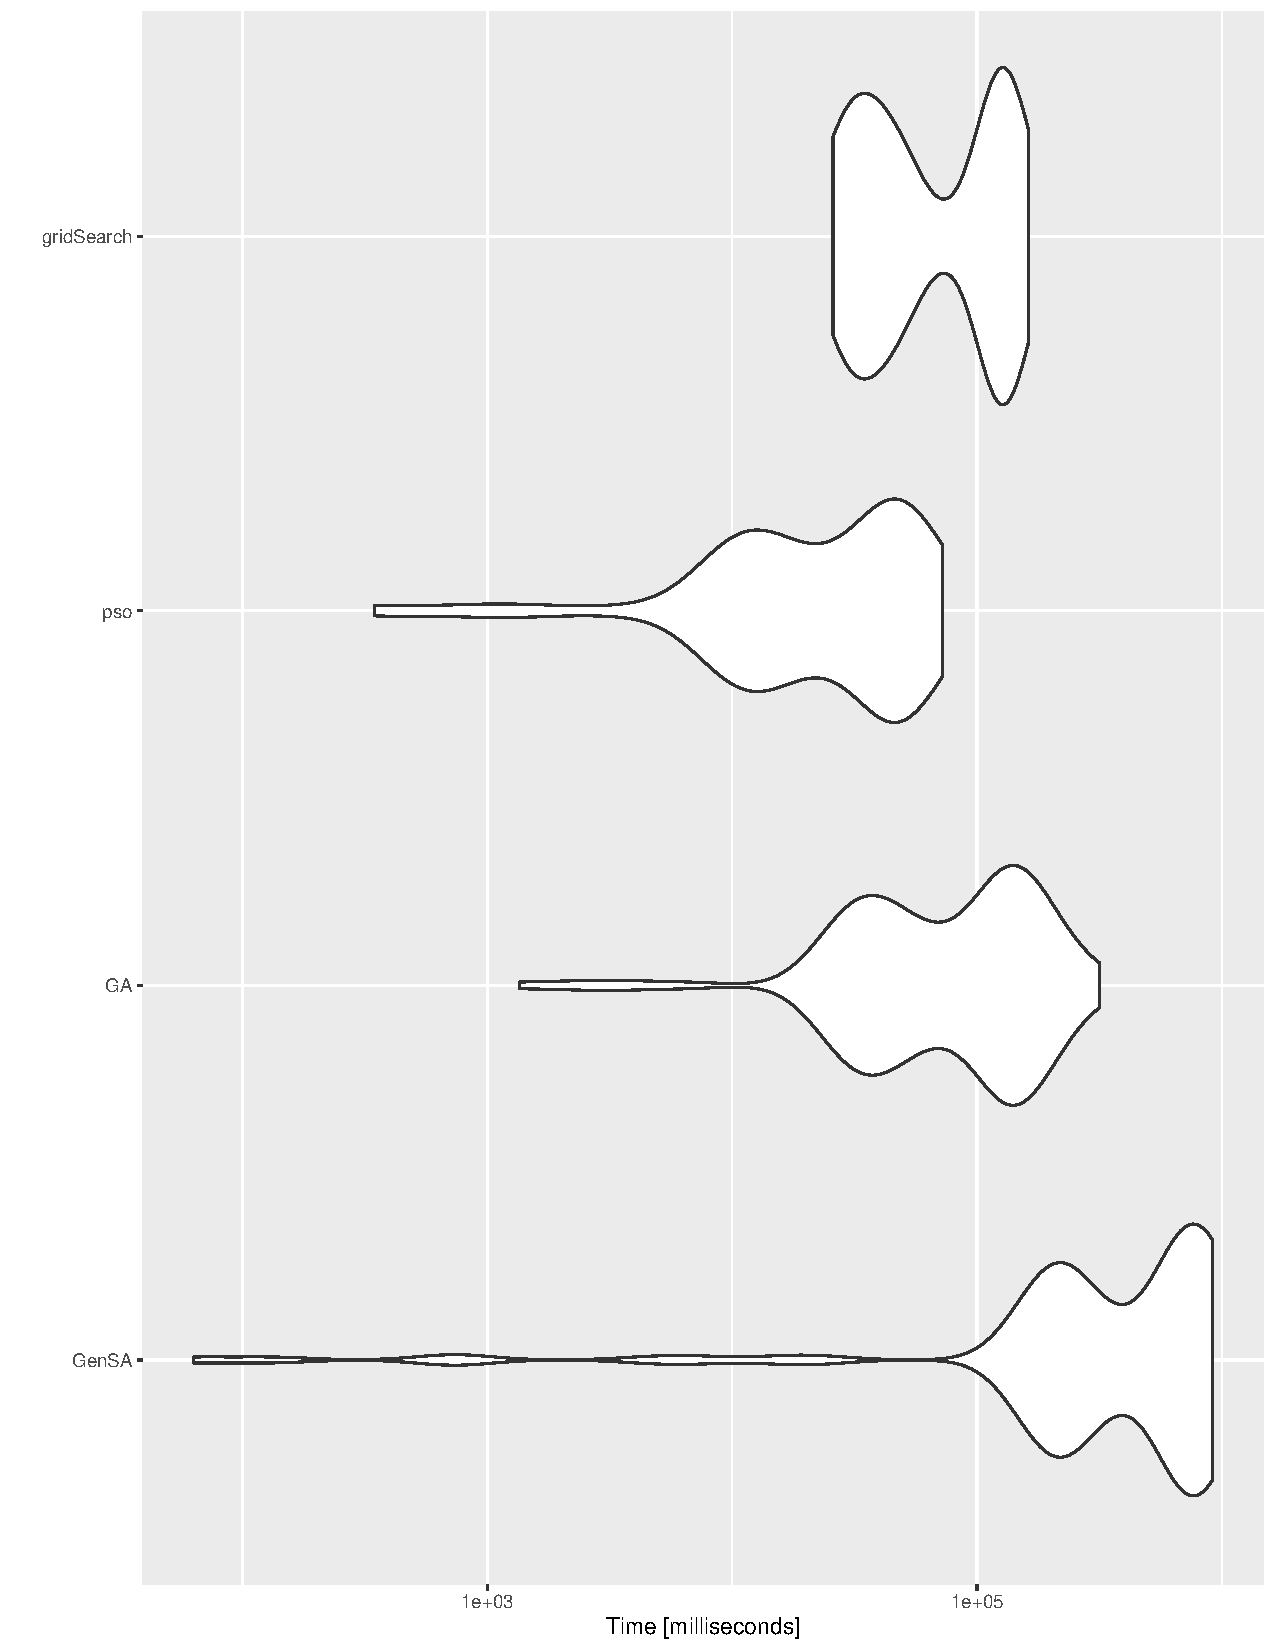
\includegraphics[width=0.9\linewidth]{fig/BF_compare}
\caption{Density plot for evaluation time of mmc(y = data, statistic = statistic, dgp = dgp, est = est, lower = lower, upper = upper, N = 99,	type = ``absolute'') with different global optimization algorithms}
\label{fig:bfcompare}
\end{figure}

As we can see, the \code{pso} seems to provide the most efficient method in this case. The \code{GenSA} might take on average the longest time for this example, but we also note that in some cases it finds a solution quite rapidly. Moreover, the grid search method might seem to perform well since it only evaluates the function at $10^3$ points. If we double the accuracy, the time needed would increase by a factor of 8 which would make this method ineffective compared to others. Additionally, we did not use any parallelization in the controls of the methods. As such, \code{GA} and \code{gridSearch} performance could have been improved quite significantly.

Finally, since the methods are metaheuristic, this figure is sadly not enough for us to make any comment on how efficient one method is compared to another in finding a ``good'' solution. In the end, the choice of method might boil down to personal preference. What is important regarding the \pkg{MaxMC} package is that it is able to provide any tools needed to solve any problem thrown at it.

\section{Irregular Wald tests}

In this section, we look at the problem of Wald-type tests where the regularity conditions are violated. This situation arises when the covariance matrix of the restrictions, as described in \cite{dufour_wald_2013,dufour_rank-robust_2016}, does not have full column rank in an open neighborhood of the true value of the parameter vector.

\subsection{Framework}

Let $\theta = [\theta_1,...,\theta_p]'$ and $\psi(\theta)= [\psi_1(\theta),...,\psi_q(\theta)]'$ where $q \leq p$, then we are looking to test the following set of hypotheses
\begin{align}
	H_0: \psi (\theta) & = \psi_0 \\
	H_1: \psi (\theta) & \neq \psi_0
\end{align}

Let $\bar{\theta}$ be the true parameter value, we assume that $\psi(\theta)= [\psi_1(\theta),...,\psi_q(\theta)]'$ is continuously differentiable on $\Theta$ where $\Theta$ is an open subset of $\R^p$ where $\bar{\theta}\in \Theta$.

Then the usual Wald statistic is defined as follows
\begin{align}
	W_n(\psi_0) & = n \left[\psi (\theta) - \psi_0\right]' \Sigma_\psi^{-1} \left[\psi (\theta) - \psi_0\right]
\end{align}
where $\Sigma_\psi$ is the covariance matrix of the restriction $\psi$.

Usually $\theta$ and $\Sigma_\psi$ need to be estimated and the Wald statistic is defined as
\begin{align}
	W_n(\psi_0) & = n \left[\psi (\hat{\theta}) - \psi_0\right]' \hat{\Sigma}_\psi^{-1} \left[\psi (\hat{\theta}) - \psi_0\right]
\end{align}

Note, as described in \cite{dufour_wald_2013,dufour_rank-robust_2016}, we can have two problematic situations:
\begin{enumerate}
	\item $\hat{\Sigma}_\psi$ has full rank, but convergences to a singular  $\Sigma_\psi$
	\item $\hat{\Sigma}_\psi$ does not have full rank, but $rank[\hat{\Sigma}_\psi] \neq rank[\Sigma_\psi]$
\end{enumerate}

Now, note that if we assume
\begin{align}
	\sqrt{n} ( \hat{\theta_n}- \theta ) & \xrightarrow{n \rightarrow \infty} N(0,I)
\end{align}

Then, $\hat{\Sigma}_\psi$ has form
\begin{align}
	\hat{\Sigma}_\psi & = P(\hat{\theta}) \hat{\Sigma}_\theta P(\hat{\theta})'
\end{align}
where $P(\theta)=\frac{\partial \psi}{\partial \theta'}$

Therefore, the Wald statistic can be rewritten as follows
\begin{align}
	W_n(\psi_0) & = n \left[\psi (\hat{\theta}) - \psi_0\right]' \left[ P(\hat{\theta}) \hat{\Sigma}_\theta P(\hat{\theta})' \right]^{-1} \left[\psi (\hat{\theta}) - \psi_0\right]
\end{align}

\subsection{Example 1}

This example is given by \cite{dufour_rank-robust_2016}. It is a simple example of two restrictions, where we test
\begin{align}
	H_0: [\theta_1 \theta_2 , \theta_1]' & = 0 \\
	H_1: [\theta_1 \theta_2 , \theta_1]'  & \neq 0
\end{align}
It is easy to see that this is a simple case of redundant restrictions. In fact, both restrictions amount to testing that $\theta_1=0$.

In order to simplify the analysis of this example, we let $\hat{\Sigma}_\theta=\Sigma_\theta=I$.

Then, we have the following
\begin{align}
	P(\theta) = \left[\begin{array}{cc}
		\theta_2 & \theta_1 \\
		1 & 0
	\end{array}\right]
\end{align}
and
\begin{align}
	P(\hat{\theta})\Sigma_\theta P(\hat{\theta})' = \left[\begin{array}{cc}
		\hat{\theta}_1^2 + \hat{\theta}_2^2 & \hat{\theta}_2 \\
		\hat{\theta}_2 & 1
	\end{array}\right]
\end{align}

Then, we have
\begin{align}
	P(\hat{\theta})\Sigma_\theta P(\hat{\theta})'\xrightarrow{n \rightarrow \infty} P(\theta)\Sigma_\theta P(\theta)'
\end{align}
where $P(\theta)\Sigma_\theta P(\theta)'$ is singular.


Taking the usual Wald statistic we have the following
\begin{align}
	W_n & = n \hat{\theta}_1^2 \xrightarrow{n \rightarrow \infty} \chi^2_1
\end{align}

Consequently, compared to the usual $\chi^2$ distribution of the $W_n$, the true asymptotic distribution is then conservative.

\subsubsection{Simulation study}
\paragraph{Level}

First, we start by simulating $\hat{\theta_1} \sim N(\theta_1,\frac{1}{n})$, $\hat{\theta_2} \sim N(\theta_2,\frac{1}{n})$, where $n$ is the sample size and $\theta_1=0$, for different values of $\theta_2$. The empirical levels for the Wald statistic are reported in table \ref{tbl:W:1}. Note that since the distribution of the statistic is not dependent on any nuisance parameter, the MMC is not directly applicable. Therefore, we only report the result for the asymptotic test and the LMC.

\begin{table}[H]
	\centering
	\scalebox{0.9}{
		\begin{tabular}{|r|r|r|r|r|r|r|r|r|r|r|}
			\hline
			& \multicolumn{2}{|c|}{$\theta_2=0$} & \multicolumn{2}{|c|}{$\theta_2=\frac{1}{4}$} & \multicolumn{2}{|c|}{$\theta_2=\frac{1}{2}$} & \multicolumn{2}{|c|}{$\theta_2=1$} & \multicolumn{2}{|c|}{$\theta_2=5$} \\ \hline
			Size & Asy & LMC & Asy & LMC & Asy & LMC & Asy & LMC & Asy & LMC  \\
			\hline
			15 & 2.4 & 6.0 & 1.2 & 5.6 & 1.6 & 5.6 & 0.8 & 4.0 & 1.6 & 4.0 \\
			25 & 2.8 & 6.0 & 1.2 & 4.0 & 1.6 & 3.6 & 2.0 & 6.8 & 2.8 & 6.8 \\
			50 & 1.2 & 4.4 & 1.2 & 3.6 & 1.2 & 4.8 & 2.0 & 2.8 & 1.6 & 8.0 \\
			100 & 1.6 & 4.4 & 2.4 & 6.4 & 0.8 & 3.6 & 0.8 & 5.2 & 2.4 & 6.0 \\
			150 & 2.8 & 4.8 & 2.4 & 4.8 & 1.6 & 5.2 & 0.8 & 4.8 & 1.2 & 3.6 \\
			200 & 1.2 & 5.2 & 0.8 & 4.0 & 3.2 & 5.2 & 0.8 & 4.8 & 2.4 & 5.2 \\
			250 & 0.4 & 6.0 & 0.8 & 4.4 & 1.6 & 4.4 & 0.4 & 2.4 & 1.6 & 4.4 \\
			300 & 2.8 & 5.2 & 4.0 & 5.6 & 0.8 & 3.6 & 0.8 & 4.0 & 1.6 & 5.2 \\
			\hline
		\end{tabular}
	}
	\caption{Empirical levels for 1000 replications of the Wald statistic where $\alpha = 5\%$ and $\theta_1=0$, testing $H_0: \left[ \theta_1\theta_2, \theta_1\right] =0$ against $H_1: \left[ \theta_1\theta_2, \theta_1\right] \neq 0$}
	\label{tbl:W:1}
\end{table}


As expected, the empirical level shows that the asymptotic test under-rejects in all cases. The LMC result seems to oscillate around the 5\% nominal level, but sometimes over-rejecting (e.g. 8\% in the case of $\theta_2= 5 $ and $n=50$).

\paragraph{Power}

Now, we test for the power of the Wald statistic based on $\chi_2^2$ critical values and the LMC, by simulating the test statistic under the alternative by picking different values for $\theta_1\neq 0$ (e.g. $\theta_1=\frac{1}{4},\frac{1}{2},1$). The empirical levels are reported in table \ref{tbl:W:2}, \ref{tbl:W:3} and \ref{tbl:W:4}.

\begin{table}[H]
	\centering
	\scalebox{0.9}{
		\begin{tabular}{|r|r|r|r|r|r|r|r|r|r|r|}
			\hline
			& \multicolumn{2}{|c|}{$\theta_2=0$} & \multicolumn{2}{|c|}{$\theta_2=\frac{1}{4}$} & \multicolumn{2}{|c|}{$\theta_2=\frac{1}{2}$} & \multicolumn{2}{|c|}{$\theta_2=1$} & \multicolumn{2}{|c|}{$\theta_2=5$} \\ \hline
			Size & Asy & LMC & Asy & LMC & Asy & LMC & Asy & LMC & Asy & LMC  \\
			\hline
			15 & 6.8 & 16.0 & 10.0 & 18.0 & 8.0 & 16.4 & 6.8 & 15.6 & 6.8 & 16.4 \\
			25 & 12.8 & 24.4 & 10.8 & 18.0 & 11.6 & 24.8 & 12.4 & 24.0 & 11.2 & 27.2 \\
			50 & 25.2 & 41.6 & 20.4 & 36.4 & 20.8 & 42.4 & 24.0 & 43.6 & 27.2 & 42.8 \\
			100 & 52.0 & 72.8 & 52.0 & 64.8 & 46.8 & 66.8 & 50.4 & 64.4 & 50.0 & 66.8 \\
			150 & 73.2 & 84.8 & 78.4 & 87.2 & 72.4 & 85.2 & 71.6 & 85.2 & 77.2 & 89.2 \\
			200 & 88.0 & 92.8 & 88.0 & 94.8 & 84.4 & 93.2 & 82.0 & 90.0 & 87.2 & 91.2 \\
			250 & 95.2 & 98.8 & 92.0 & 96.8 & 91.6 & 96.8 & 93.2 & 97.2 & 93.6 & 96.4 \\
			300 & 97.2 & 98.8 & 98.4 & 99.2 & 95.6 & 98.0 & 97.6 & 99.2 & 96.0 & 98.8 \\
			\hline
		\end{tabular}
	}
	\caption{Empirical levels for 1000 replications of the Wald statistic where $\alpha = 5\%$ and $\theta_1=\frac{1}{4}$, testing $H_0: \left[ \theta_1\theta_2, \theta_1\right] =0$ against $H_1: \left[ \theta_1\theta_2, \theta_1\right] \neq 0$}
	\label{tbl:W:2}
\end{table}

\begin{table}[H]
	\centering
	\scalebox{0.9}{
		\begin{tabular}{|r|r|r|r|r|r|r|r|r|r|r|}
			\hline
			& \multicolumn{2}{|c|}{$\theta_2=0$} & \multicolumn{2}{|c|}{$\theta_2=\frac{1}{4}$} & \multicolumn{2}{|c|}{$\theta_2=\frac{1}{2}$} & \multicolumn{2}{|c|}{$\theta_2=1$} & \multicolumn{2}{|c|}{$\theta_2=5$} \\ \hline
			Size & Asy & LMC & Asy & LMC & Asy & LMC & Asy & LMC & Asy & LMC  \\
			\hline
			15 & 32.4 & 44.0 & 34.4 & 54.8 & 32.8 & 50.8 & 26.0 & 44.0 & 29.6 & 52.0 \\
			25 & 44.8 & 62.8 & 53.2 & 72.0 & 53.2 & 72.0 & 54.0 & 70.8 & 58.4 & 67.6 \\
			50 & 80.8 & 90.0 & 82.0 & 92.8 & 90.4 & 96.8 & 86.4 & 92.8 & 92.0 & 96.0 \\
			100 & 100.0 & 100.0 & 100.0 & 100.0 & 99.6 & 100.0 & 100.0 & 100.0 & 99.6 & 100.0 \\
			150 & 100.0 & 100.0 & 100.0 & 100.0 & 100.0 & 100.0 & 100.0 & 100.0 & 100.0 & 100.0 \\
			200 & 100.0 & 100.0 & 100.0 & 100.0 & 100.0 & 100.0 & 100.0 & 100.0 & 100.0 & 100.0 \\
			250 & 100.0 & 100.0 & 100.0 & 100.0 & 100.0 & 100.0 & 100.0 & 100.0 & 100.0 & 100.0 \\
			300 & 100.0 & 100.0 & 100.0 & 100.0 & 100.0 & 100.0 & 100.0 & 100.0 & 100.0 & 100.0 \\
			\hline
		\end{tabular}
	}
	\caption{Empirical levels for 1000 replications of the Wald statistic where $\alpha = 5\%$ and $\theta_1=\frac{1}{2}$, testing $H_0: \left[ \theta_1\theta_2, \theta_1\right] =0$ against $H_1: \left[ \theta_1\theta_2, \theta_1\right] \neq 0$}
	\label{tbl:W:3}
\end{table}

\begin{table}[H]
	\centering
	\scalebox{0.9}{
		\begin{tabular}{|r|r|r|r|r|r|r|r|r|r|r|}
			\hline
			& \multicolumn{2}{|c|}{$\theta_2=0$} & \multicolumn{2}{|c|}{$\theta_2=\frac{1}{4}$} & \multicolumn{2}{|c|}{$\theta_2=\frac{1}{2}$} & \multicolumn{2}{|c|}{$\theta_2=1$} & \multicolumn{2}{|c|}{$\theta_2=5$} \\ \hline
			Size & Asy & LMC & Asy & LMC & Asy & LMC & Asy & LMC & Asy & LMC  \\
			\hline
			15 & 94 & 98.4 & 91.6 & 98 & 94.8 & 97.2 & 94.0 & 99.2 & 91.6 & 96.4 \\
			25 & 100 & 100.0 & 99.6 & 100 & 99.6 & 100.0 & 99.2 & 99.6 & 99.6 & 99.6 \\
			50 & 100 & 100.0 & 100.0 & 100 & 100.0 & 100.0 & 100.0 & 100.0 & 100.0 & 100.0 \\
			100 & 100 & 100.0 & 100.0 & 100 & 100.0 & 100.0 & 100.0 & 100.0 & 100.0 & 100.0 \\
			150 & 100 & 100.0 & 100.0 & 100 & 100.0 & 100.0 & 100.0 & 100.0 & 100.0 & 100.0 \\
			200 & 100 & 100.0 & 100.0 & 100 & 100.0 & 100.0 & 100.0 & 100.0 & 100.0 & 100.0 \\
			250 & 100 & 100.0 & 100.0 & 100 & 100.0 & 100.0 & 100.0 & 100.0 & 100.0 & 100.0 \\
			300 & 100 & 100.0 & 100.0 & 100 & 100.0 & 100.0 & 100.0 & 100.0 & 100.0 & 100.0 \\
			\hline
		\end{tabular}
	}
	\caption{Empirical levels for 1000 replications of the Wald statistic where $\alpha = 5\%$ and $\theta_1=1$, testing $H_0: \left[ \theta_1\theta_2, \theta_1\right] =0$ against $H_1: \left[ \theta_1\theta_2, \theta_1\right] \neq 0$}
	\label{tbl:W:4}
\end{table}


It is clear from tables \ref{tbl:W:2}, \ref{tbl:W:3} and \ref{tbl:W:4}, that the simulation based method has a consistently higher power. This is as expected, since the asymptotic test based on $\chi_2^2$ critical values should be conservative, therefore reducing both the level and power of the test.

Additionally, we note that as $\theta_1$ diverges from the null hypothesis (i.e. $\theta_1=0$), the power of both test increase.

\subsection{Example 2}
The following example is given by \cite{dufour_wald_2013}. We are looking to test the following set of hypotheses
\begin{align}
	H_0: \theta_1^2+...+\theta_p^2 & = 0 \\
	H_1: \theta_1^2+...+\theta_p^2  & \neq 0
\end{align}

Again, we let $\hat{\Sigma}_\theta=\Sigma_\theta=I$. Then, under $H_0$, we have $\theta_1=...=\theta_p=0$ and the following derivative matrix
\begin{align}
	P(\theta) = \left[2\theta_1, ... , 2\theta_p \right]
\end{align}

Hence, the asymptotic covariance matrix of the restriction reduces to
\begin{align}
	P(\hat{\theta})\hat{\Sigma}_\theta P(\hat{\theta})' = 4(\hat{\theta}_1^2+...+\hat{\theta}_p^2)
\end{align}
where
\begin{align}
	P(\hat{\theta})\hat{\Sigma}_\theta P(\hat{\theta})'\xrightarrow{n \rightarrow \infty} 0
\end{align}

Therefore, the regularity condition is violated and we have the following Wald statistic
\begin{align}
	W_n & = \frac{n}{4}( \hat{\theta}_1^2 + ... + \hat{\theta}_p^2) = \frac{n}{4} \sum_{i=1}^{p}\hat{\theta}_i^2
\end{align}

It is then easy to see that
\begin{align}
	W_n & \xrightarrow{n \rightarrow \infty}\frac{1}{4} \chi^2_p
\end{align}
which implies that the test might lead to under-rejection for low $p$ and severe over-rejection for high $p$.

\subsubsection{Simulation study}
\paragraph{Level}

We simulate $\hat{\theta_i} \sim N(0,\frac{1}{n})$ for $i=1,...p$, where $p$ is the number of parameters in the restriction. The empirical levels are reported in table \ref{tbl:W:5}.

\begin{table}[H]
	\centering
	\scalebox{0.9}{
		\begin{tabular}{|r|r|r|r|r|r|r|r|r|r|r|}
			\hline
			& \multicolumn{2}{|c|}{$p=2$} & \multicolumn{2}{|c|}{$p=5$} & \multicolumn{2}{|c|}{$p=10$} & \multicolumn{2}{|c|}{$p=20$} & \multicolumn{2}{|c|}{$p=30$} \\ \hline
			Size & Asy & LMC & Asy & LMC & Asy & LMC & Asy & LMC & Asy & LMC  \\
			\hline
			15 & 0 & 1.2 & 0 & 2.8 & 0.4 & 2.4 & 24.0 & 3.2 & 75.2 & 1.2 \\
			25 & 0 & 4.0 & 0 & 1.6 & 0.8 & 3.6 & 18.4 & 1.6 & 78.4 & 3.2 \\
			50 & 0 & 2.4 & 0 & 2.4 & 1.6 & 3.2 & 23.6 & 2.8 & 79.2 & 4.8 \\
			100 & 0 & 2.4 & 0 & 3.6 & 0.4 & 2.4 & 25.6 & 4.8 & 76.8 & 2.4 \\
			150 & 0 & 2.8 & 0 & 2.0 & 1.2 & 2.8 & 21.6 & 2.8 & 76.4 & 3.6 \\
			200 & 0 & 2.0 & 0 & 2.8 & 0.4 & 2.8 & 24.8 & 2.0 & 72.4 & 5.6 \\
			250 & 0 & 2.8 & 0 & 1.6 & 0.0 & 0.8 & 18.8 & 3.2 & 74.8 & 5.2 \\
			300 & 0 & 2.4 & 0 & 2.8 & 0.0 & 4.4 & 22.8 & 4.8 & 77.2 & 4.8 \\
			\hline
		\end{tabular}
	}
	\caption{Empirical levels for 1000 replications of the Wald statistic where $\alpha = 5\%$, $\theta_1=0$ and $\theta_2=...=\theta_p=0$,  testing $H_0: \theta_1^2 + ...  +\theta_p^2 =0$ against $H_1: \theta_1^2 + ...  +\theta_p^2  \neq 0$}
	\label{tbl:W:5}
\end{table}


First, looking at the LMC, we see that we almost always under reject. More precisely, the empirical levels range from 1.2\% to 5.6\% for the LMC.

The really interesting part of this example is how the asymptotic test starts off by severely under-rejecting for low values of $p$ (e.g. $p=2,5,10$), and then starts to over-reject as $p$ increases. In fact, for $p=30$, the asymptotic test empirical levels are around 75\% for a 5\% level test. While in the previous example one might have chosen the asymptotic test without any severe consequence on the level of the test, in this example it is quite the opposite.

\paragraph{Power}

In this section, we let $\theta_1$ vary from the null hypothesis that $\theta_1=0$. Results for the empirical levels when $\hat{\theta}$ is generated under the alternative are reported in tables \ref{tbl:W:6}, \ref{tbl:W:7} and  \ref{tbl:W:8}.

\begin{table}[H]
	\centering
	\scalebox{0.9}{
		\begin{tabular}{|r|r|r|r|r|r|r|r|r|r|r|}
			\hline
			& \multicolumn{2}{|c|}{$p=2$} & \multicolumn{2}{|c|}{$p=5$} & \multicolumn{2}{|c|}{$p=10$} & \multicolumn{2}{|c|}{$p=20$} & \multicolumn{2}{|c|}{$p=30$} \\ \hline
			Size & Asy & LMC & Asy & LMC & Asy & LMC & Asy & LMC & Asy & LMC  \\
			\hline
			15 & 0.0 & 7.2 & 0.0 & 5.2 & 2.4 & 6.0 & 31.6 & 5.6 & 81.2 & 4.8 \\
			25 & 0.0 & 12.4 & 0.0 & 8.4 & 2.8 & 8.4 & 28.4 & 5.6 & 82.4 & 8.4 \\
			50 & 0.0 & 16.8 & 0.8 & 16.0 & 7.6 & 14.8 & 38.0 & 6.0 & 88.0 & 7.6 \\
			100 & 2.0 & 42.0 & 2.8 & 33.6 & 11.2 & 26.8 & 57.2 & 18.4 & 90.8 & 18.8 \\
			150 & 4.4 & 61.2 & 7.6 & 53.6 & 23.6 & 47.2 & 71.2 & 33.6 & 96.0 & 29.2 \\
			200 & 7.6 & 80.8 & 17.2 & 66.0 & 39.2 & 59.2 & 80.8 & 45.2 & 98.4 & 39.6 \\
			250 & 22.4 & 90.0 & 33.2 & 82.8 & 59.6 & 75.2 & 90.8 & 66.4 & 99.2 & 47.6 \\
			300 & 32.8 & 96.4 & 44.8 & 88.4 & 70.0 & 85.2 & 92.8 & 63.6 & 100.0 & 60.4 \\
			\hline
		\end{tabular}
	}
	\caption{Empirical levels for 1000 replications of the Wald statistic where $\alpha = 5\%$, $\theta_1=\frac{1}{4}$ and $\theta_2=...=\theta_p=0$,  testing $H_0: \theta_1^2 + ...  +\theta_p^2 =0$ against $H_1: \theta_1^2 + ...  +\theta_p^2  \neq 0$}
	\label{tbl:W:6}
\end{table}

\begin{table}[H]
	\centering
	\scalebox{0.9}{
		\begin{tabular}{|r|r|r|r|r|r|r|r|r|r|r|}
			\hline
			& \multicolumn{2}{|c|}{$p=2$} & \multicolumn{2}{|c|}{$p=5$} & \multicolumn{2}{|c|}{$p=10$} & \multicolumn{2}{|c|}{$p=20$} & \multicolumn{2}{|c|}{$p=30$} \\ \hline
			Size & Asy & LMC & Asy & LMC & Asy & LMC & Asy & LMC & Asy & LMC  \\
			\hline
			15 & 0.0 & 27.6 & 1.2 & 20.8 & 6.4 & 16.8 & 44.0 & 11.2 & 88.0 & 10.4 \\
			25 & 0.4 & 41.6 & 1.6 & 34.4 & 12.4 & 25.2 & 59.6 & 22.8 & 91.6 & 17.2 \\
			50 & 11.2 & 82.0 & 18.8 & 73.2 & 38.4 & 60.4 & 78.8 & 43.2 & 98.0 & 39.2 \\
			100 & 56.0 & 97.6 & 68.8 & 96.0 & 83.6 & 92.4 & 98.8 & 85.6 & 100.0 & 78.8 \\
			150 & 88.0 & 99.6 & 93.6 & 100.0 & 97.2 & 99.6 & 100.0 & 97.2 & 100.0 & 96.8 \\
			200 & 99.2 & 100.0 & 98.8 & 100.0 & 100.0 & 100.0 & 100.0 & 99.6 & 100.0 & 99.6 \\
			250 & 99.6 & 100.0 & 100.0 & 100.0 & 100.0 & 100.0 & 100.0 & 100.0 & 100.0 & 100.0 \\
			300 & 100.0 & 100.0 & 100.0 & 100.0 & 100.0 & 100.0 & 100.0 & 100.0 & 100.0 & 100.0 \\
			\hline
		\end{tabular}
	}
	\caption{Empirical levels for 1000 replications of the Wald statistic where $\alpha = 5\%$, $\theta_1=\frac{1}{2}$ and $\theta_2=...=\theta_p=0$,  testing $H_0: \theta_1^2 + ...  +\theta_p^2 =0$ against $H_1: \theta_1^2 + ...  +\theta_p^2  \neq 0$}
	\label{tbl:W:7}
\end{table}

\begin{table}[H]
	\centering
	\scalebox{0.9}{
		\begin{tabular}{|r|r|r|r|r|r|r|r|r|r|r|}
			\hline
			& \multicolumn{2}{|c|}{$p=2$} & \multicolumn{2}{|c|}{$p=5$} & \multicolumn{2}{|c|}{$p=10$} & \multicolumn{2}{|c|}{$p=20$} & \multicolumn{2}{|c|}{$p=30$} \\ \hline
			Size & Asy & LMC & Asy & LMC & Asy & LMC & Asy & LMC & Asy & LMC  \\
			\hline
			15 & 18.8 & 90.4 & 28.4 & 80.8 & 52.0 & 69.2 & 86.0 & 58.4 & 97.6 & 46.0 \\
			25 & 60.8 & 98.8 & 70.4 & 96.0 & 86.8 & 96.0 & 97.6 & 84.4 & 100.0 & 78.4 \\
			50 & 97.6 & 100.0 & 98.8 & 100.0 & 100.0 & 100.0 & 100.0 & 99.6 & 100.0 & 99.6 \\
			100 & 100.0 & 100.0 & 100.0 & 100.0 & 100.0 & 100.0 & 100.0 & 100.0 & 100.0 & 100.0 \\
			150 & 100.0 & 100.0 & 100.0 & 100.0 & 100.0 & 100.0 & 100.0 & 100.0 & 100.0 & 100.0 \\
			200 & 100.0 & 100.0 & 100.0 & 100.0 & 100.0 & 100.0 & 100.0 & 100.0 & 100.0 & 100.0 \\
			250 & 100.0 & 100.0 & 100.0 & 100.0 & 100.0 & 100.0 & 100.0 & 100.0 & 100.0 & 100.0 \\
			300 & 100.0 & 100.0 & 100.0 & 100.0 & 100.0 & 100.0 & 100.0 & 100.0 & 100.0 & 100.0 \\
			\hline
		\end{tabular}
	}
	\caption{Empirical levels for 1000 replications of the Wald statistic where $\alpha = 5\%$, $\theta_1=1$ and $\theta_2=...=\theta_p=0$,  testing $H_0: \theta_1^2 + ...  +\theta_p^2 =0$ against $H_1: \theta_1^2 + ...  +\theta_p^2  \neq 0$}
	\label{tbl:W:8}
\end{table}



Looking at tables \ref{tbl:W:6}, \ref{tbl:W:7} and  \ref{tbl:W:8}, we see that, while the power of LMC seems to be constant over different values of $p$, as $n$ increases, so does the power of the LMC test.

Now for the asymptotic test, when $p$ is low, the power of the test is low compared to the LMC. When $p$ is high, then the power of the test is close to 100\% even for low $n$ and $\theta_1$ close to 0. This feature is simply a consequence of the nature of the test statistic, where the $\chi_p^2$ critical values are conservative when $p$ is low and untrustworthy when $p$ is high.

\subsection{Example 3}

The following example is again given by \cite{dufour_wald_2013}. It is again a case of redundant restrictions like the example 1, but where
\begin{align}
	H_0: [\theta_1 \theta_2^2 , \theta_1^2]' & = 0 \\
	H_1: [\theta_1 \theta_2^2 , \theta_1^2]'  & \neq 0
\end{align}

Therefore, both restrictions can be reduced to the restriction that $\theta_1=0$. This in turns leads to the following derivative matrix
\begin{align}
	P(\theta) = \left[\begin{array}{cc}
		\theta_2^2 & 2\theta_1 \theta_2 \\
		2\theta_1 & 0
	\end{array}\right]
\end{align}

Then, for $\hat{\Sigma}_\theta=\Sigma_\theta=I$, we have
\begin{align}
	P(\hat{\theta})\hat{\Sigma}_\theta P(\hat{\theta})' = \left[\begin{array}{cc}
		\hat{\theta}_2^4 + 4 \hat{\theta}_1^2\hat{\theta}_2^2 &  2 \hat{\theta}_1\hat{\theta}_2^2 \\
		2 \hat{\theta}_1\hat{\theta}_2^2&  4 \hat{\theta}_1^2
	\end{array}\right]
\end{align}
and it is easy to see that, as $n\rightarrow\infty$, the asymptotic covariance matrix converges to a singular one.

Wald-statistic is then
\begin{align}
	W_n & = \frac{n}{16}(4 \hat{\theta}_1^2 + \hat{\theta}_2^2)
\end{align}

This leads the following two cases \begin{itemize}
	\item[Case 1:] $\theta_1=0$ and $ \theta_2 = 0$

	\begin{align}
		W_n & \xrightarrow{n \rightarrow \infty} \frac{1}{4} Z_1^2 + \frac{1}{16} Z_2^2 \leq \frac{1}{4}( Z_1^2 + Z_2^2) \sim \frac{1}{4} \chi^2_2
	\end{align}

	\item[Case 2:] $\theta_1=0$ and $ \theta_2 \neq 0$
	\begin{align}
		W_n & \xrightarrow{n \rightarrow \infty} + \infty
	\end{align}
\end{itemize}

Since the usual Wald-statistic would use $\chi^2_2$ critical values to test $H_0$, it is easy to see that under case 1, the test would be conservative, while under case 2, it would dangerously over-reject.


\subsubsection{Simulation study}
\paragraph{Level}

As for the example 1, we simulate $\hat{\theta_1} \sim N(\theta_1,\frac{1}{n})$, $\hat{\theta_2} \sim N(\theta_2,\frac{1}{n})$, where $n$ is the sample size and $\theta_1=0$, for different values of $\theta_2$. The empirical levels are reported in table \ref{tbl:W:9}. Note that since $\theta_2$ is a nuisance parameter, the MMC is always reported along the asymptotic test and the LMC. Note that for the MMC, we build a 99\% confidence interval using maximum likelihood for $\theta_2$ and test the p-value against a level of 4\%. Then, this two-stage procedure should yield an exact test at the 5\% level.

\begin{table}[H]
	\centering
	\scalebox{0.65}{
		\begin{tabular}{|r|r|r|r|r|r|r|r|r|r|r|r|r|r|r|r|}
			\hline
			& \multicolumn{3}{|c|}{$\theta_2=0$} & \multicolumn{3}{|c|}{$\theta_2=\frac{1}{4}$} & \multicolumn{3}{|c|}{$\theta_2=\frac{1}{2}$} & \multicolumn{3}{|c|}{$\theta_2=1$} & \multicolumn{3}{|c|}{$\theta_2=5$} \\ \hline
			Size & Asy & LMC  & MMC & Asy & LMC  & MMC & Asy & LMC & MMC & Asy & LMC & MMC & Asy & LMC & MMC  \\
			\hline
			15 & 0 & 3.8 & 0.6 & 0 & 4.1 & 0.4 & 0.0 & 3.0 & 0.1 & 0.0 & 1.2 & 0 & 100 & 0 & 0 \\
			25 & 0 & 3.8 & 0.6 & 0 & 3.5 & 0.2 & 0.0 & 2.7 & 0.1 & 0.0 & 1.0 & 0 & 100 & 0 & 0 \\
			50 & 0 & 3.8 & 0.6 & 0 & 3.0 & 0.1 & 0.0 & 1.5 & 0.0 & 1.0 & 0.4 & 0 & 100 & 0 & 0 \\
			100 & 0 & 3.8 & 0.6 & 0 & 2.7 & 0.1 & 0.0 & 1.0 & 0.0 & 67.0 & 0.1 & 0 & 100 & 0 & 0 \\
			150 & 0 & 3.8 & 0.6 & 0 & 1.9 & 0.1 & 0.2 & 0.5 & 0.0 & 99.7 & 0.1 & 0 & 100 & 0 & 0 \\
			200 & 0 & 3.8 & 0.6 & 0 & 1.5 & 0.0 & 1.0 & 0.4 & 0.0 & 100.0 & 0.1 & 0 & 100 & 0 & 0 \\
			250 & 0 & 3.8 & 0.6 & 0 & 1.1 & 0.0 & 5.9 & 0.2 & 0.0 & 100.0 & 0.0 & 0 & 100 & 0 & 0 \\
			\hline
		\end{tabular}
	}
	\caption{Empirical levels for 1000 replications of the Wald statistic where $\alpha = 5\%$, $\theta_1=0$, testing $H_0: \left[ \theta_1\theta_2^2, \theta_1^2\right] =0$ against $H_1: \left[ \theta_1\theta_2^2, \theta_1^2\right] \neq 0$}
	\label{tbl:W:9}
\end{table}


In this example, every test under-rejects. What is interesting is that, as $\theta_2$ increases, the LMC and MMC empirical go down even further, but the asymptotic starts to severely over-reject even when $\theta_2=1$. This point suggests that the traditional critical values are misleading in this example.

\paragraph{Power}

Results for empirical levels when $\theta_1\neq 0$ are reported in tables \ref{tbl:W:10}, \ref{tbl:W:11} and  \ref{tbl:W:12}.

\begin{table}[H]
	\centering
	\scalebox{0.65}{
		\begin{tabular}{|r|r|r|r|r|r|r|r|r|r|r|r|r|r|r|r|}
			\hline
			& \multicolumn{3}{|c|}{$\theta_2=0$} & \multicolumn{3}{|c|}{$\theta_2=\frac{1}{4}$} & \multicolumn{3}{|c|}{$\theta_2=\frac{1}{2}$} & \multicolumn{3}{|c|}{$\theta_2=1$} & \multicolumn{3}{|c|}{$\theta_2=5$} \\ \hline
			Size & Asy & LMC  & MMC & Asy & LMC  & MMC & Asy & LMC & MMC & Asy & LMC & MMC & Asy & LMC & MMC  \\
			\hline
			15 & 0.0 & 12.8 & 2.0 & 0.0 & 12.4 & 2.0 & 0.0 & 12.4 & 2.0 & 0.4 & 8.0 & 1.2 & 100 & 0.4 & 0 \\
			25 & 0.0 & 20.4 & 5.2 & 0.0 & 22.0 & 5.6 & 0.0 & 16.0 & 1.2 & 0.4 & 6.8 & 0.4 & 100 & 0.4 & 0 \\
			50 & 0.0 & 35.2 & 10.4 & 0.4 & 31.6 & 9.2 & 0.0 & 28.0 & 4.4 & 6.4 & 9.6 & 0.4 & 100 & 0.4 & 0 \\
			100 & 0.8 & 66.4 & 34.8 & 1.2 & 56.0 & 21.6 & 7.2 & 50.0 & 6.4 & 88.0 & 21.2 & 0.4 & 100 & 0.0 & 0 \\
			150 & 4.4 & 82.4 & 57.2 & 4.4 & 82.4 & 26.8 & 27.6 & 62.0 & 11.2 & 100.0 & 30.4 & 0.8 & 100 & 0.0 & 0 \\
			200 & 7.2 & 89.6 & 70.4 & 18.8 & 89.2 & 45.2 & 54.8 & 72.0 & 12.0 & 100.0 & 39.2 & 1.6 & 100 & 0.0 & 0 \\
			250 & 15.2 & 95.2 & 82.4 & 27.6 & 90.8 & 54.0 & 82.4 & 84.0 & 16.0 & 100.0 & 43.6 & 0.8 & 100 & 0.0 & 0 \\
			\hline
		\end{tabular}
	}
	\caption{Empirical levels for 250 replications of the Wald statistic where $\alpha = 5\%$, $\theta_1=\frac{1}{4}$, testing $H_0: \left[ \theta_1\theta_2^2, \theta_1^2\right] =0$ against $H_1: \left[ \theta_1\theta_2^2, \theta_1^2\right] \neq 0$}
	\label{tbl:W:10}
\end{table}

\begin{table}[H]
	\centering
	\scalebox{0.65}{
		\begin{tabular}{|r|r|r|r|r|r|r|r|r|r|r|r|r|r|r|r|}
			\hline
			& \multicolumn{3}{|c|}{$\theta_2=0$} & \multicolumn{3}{|c|}{$\theta_2=\frac{1}{4}$} & \multicolumn{3}{|c|}{$\theta_2=\frac{1}{2}$} & \multicolumn{3}{|c|}{$\theta_2=1$} & \multicolumn{3}{|c|}{$\theta_2=5$} \\ \hline
			Size & Asy & LMC  & MMC & Asy & LMC  & MMC & Asy & LMC & MMC & Asy & LMC & MMC & Asy & LMC & MMC  \\
			\hline
			15 & 0.0 & 38.8 & 17.2 & 0.0 & 40.0 & 11.2 & 0.0 & 33.2 & 8.8 & 0.8 & 33.6 & 3.6 & 100 & 1.6 & 0 \\
			25 & 0.8 & 66.4 & 34.8 & 0.4 & 62.8 & 26.0 & 1.2 & 56.0 & 21.6 & 7.2 & 50.0 & 6.4 & 100 & 2.4 & 0 \\
			50 & 7.2 & 89.6 & 70.4 & 10.4 & 88.4 & 64.8 & 18.8 & 89.2 & 45.2 & 54.8 & 72.0 & 12.0 & 100 & 3.6 & 0 \\
			100 & 54.0 & 99.6 & 97.6 & 59.2 & 100.0 & 94.4 & 76.8 & 99.2 & 77.6 & 100.0 & 97.6 & 42.0 & 100 & 7.2 & 0 \\
			150 & 88.0 & 100.0 & 100.0 & 90.0 & 100.0 & 100.0 & 98.8 & 100.0 & 97.2 & 100.0 & 100.0 & 67.6 & 100 & 9.2 & 0 \\
			200 & 98.0 & 100.0 & 100.0 & 98.8 & 100.0 & 100.0 & 100.0 & 100.0 & 98.8 & 100.0 & 100.0 & 88.8 & 100 & 20.4 & 0 \\
			250 & 99.6 & 100.0 & 100.0 & 100.0 & 100.0 & 100.0 & 100.0 & 100.0 & 99.6 & 100.0 & 100.0 & 94.8 & 100 & 38.4 & 0 \\
			\hline
		\end{tabular}
	}
	\caption{Empirical levels for 250 replications of the Wald statistic where $\alpha = 5\%$, $\theta_1=\frac{1}{2}$, testing $H_0: \left[ \theta_1\theta_2^2, \theta_1^2\right] =0$ against $H_1: \left[ \theta_1\theta_2^2, \theta_1^2\right] \neq 0$}
	\label{tbl:W:11}
\end{table}


\begin{table}[H]
	\centering
	\scalebox{0.65}{
		\begin{tabular}{|r|r|r|r|r|r|r|r|r|r|r|r|r|r|r|r|}
			\hline
			& \multicolumn{3}{|c|}{$\theta_2=0$} & \multicolumn{3}{|c|}{$\theta_2=\frac{1}{4}$} & \multicolumn{3}{|c|}{$\theta_2=\frac{1}{2}$} & \multicolumn{3}{|c|}{$\theta_2=1$} & \multicolumn{3}{|c|}{$\theta_2=5$} \\ \hline
			Size & Asy & LMC  & MMC & Asy & LMC  & MMC & Asy & LMC & MMC & Asy & LMC & MMC & Asy & LMC & MMC  \\
			\hline
			15 & 20 & 97.2 & 82.4 & 14.0 & 92.8 & 80.0 & 21.2 & 95.2 & 73.2 & 31.2 & 91.6 & 50.8 & 100 & 31.6 & 0.4 \\
			25 & 54 & 99.6 & 97.6 & 56.8 & 100.0 & 97.2 & 59.2 & 100.0 & 94.4 & 76.8 & 99.2 & 77.6 & 100 & 53.2 & 0.8 \\
			50 & 98 & 100.0 & 100.0 & 98.0 & 100.0 & 100.0 & 98.8 & 100.0 & 100.0 & 100.0 & 100.0 & 98.8 & 100 & 94.0 & 4.8 \\
			100 & 100 & 100.0 & 100.0 & 100.0 & 100.0 & 100.0 & 100.0 & 100.0 & 100.0 & 100.0 & 100.0 & 100.0 & 100 & 100.0 & 23.6 \\
			150 & 100 & 100.0 & 100.0 & 100.0 & 100.0 & 100.0 & 100.0 & 100.0 & 100.0 & 100.0 & 100.0 & 100.0 & 100 & 100.0 & 68.4 \\
			200 & 100 & 100.0 & 100.0 & 100.0 & 100.0 & 100.0 & 100.0 & 100.0 & 100.0 & 100.0 & 100.0 & 100.0 & 100 & 100.0 & 91.2 \\
			250 & 100 & 100.0 & 100.0 & 100.0 & 100.0 & 100.0 & 100.0 & 100.0 & 100.0 & 100.0 & 100.0 & 100.0 & 100 & 100.0 & 99.2 \\
			\hline
		\end{tabular}
	}
	\caption{Empirical levels for 250 replications of the Wald statistic where $\alpha = 5\%$, $\theta_1=1$, testing $H_0: \left[ \theta_1\theta_2^2, \theta_1^2\right] =0$ against $H_1: \left[ \theta_1\theta_2^2, \theta_1^2\right] \neq 0$}
	\label{tbl:W:12}
\end{table}


For $\theta_2$, the LMC outperfoms both the MMC and the asymptotic test. But, it is interesting to note that the MMC always performs better than the asymptotic test.

Now, difficulties start appearing when $\theta_2$ increases. As $\theta_2$ increases, the distribution of the statistic becomes more and more overpowered by this sole parameter. As such, both the LMC and MMC power goes down. The power of the MMC is more affected by this increase in $\theta_2$ since it maximizes over a confidence interval around $\hat{\theta_2}$. Note that the power of the asymptotic test increases dramatically to 100\% as $\theta_2$ increases. Again even if this might seems like a nice property to have, it is simply the result of the critical values becoming invalid for $\theta_2$.

\subsection{Example 4}

In this example, we relax the assumption that $\hat{\Sigma}_\theta=\Sigma_\theta=I$, and let
\begin{align}
	\Sigma_\theta & = \left[ \begin{array}{cc}
		1 & \rho  \\
		\rho  & 1
	\end{array} \right]
\end{align}
i.e. $\Var(\theta_1)=1$, $\Var(\theta_2)=1$ and $\Cov(\theta_1,\theta_2)=\Corr(\theta_1,\theta_2)=\rho$.

Then, we keep the same set of restrictions as the previous example i.e.
\begin{align}
	H_0: [\theta_1 \theta_2^2 , \theta_1^2]' & = 0 \\
	H_1: [\theta_1 \theta_2^2 , \theta_1^2]'  & \neq 0
\end{align}

As we recall, the Wald statistic has the following form
\begin{align}
	W_n(\psi_0) & = n \left[\psi (\hat{\theta}) - \psi_0\right]' \left[P (\hat{\theta})\Sigma_\theta P (\hat{\theta})'\right]^{-1} \left[\psi (\hat{\theta}) - \psi_0\right]
\end{align}
where in our example
\begin{align}
	P(\hat{\theta}) & = \left[ \begin{array}{cc}
		\hat{\theta}_2^2 & 2\hat{\theta}_1 \hat{\theta}_2 \\
		2\hat{\theta}_1 & 0
	\end{array} \right]
\end{align}

Therefore in this example, it reduces to
\begin{align}
	W_n & = n\left[ \frac{4\hat{\theta}_1^2-4\rho\hat{\theta}_1\hat{\theta}_2+\hat{\theta}_2^2}{16(1-\rho^2)}\right]
\end{align}
where $\Corr(\theta_1,\theta_2)=\rho$.

It is clear that the asymptotic distribution under this case is a bit more complex than in example 3. We won't go into the details of deriving the asymptotic distribution, but it is easy to see that as $\rho \rightarrow 1$, $W_n \rightarrow \infty$, which in turns implies that the usual $\chi^2_2$ critical values will over-reject the test statistic.

The problem we face is that if $\Sigma_\theta$ is not given, then we need a consistent estimator for it i.e. we need an estimator $\hat{\Sigma}_\theta$ such that
\begin{align}
	\hat{\Sigma}_\theta & \xrightarrow{n \rightarrow \infty} \Sigma_\theta
\end{align}

If we assume that we have $X_1,...,X_n$ $i.i.d.$ observations such that $X_i \sim N(\theta,\Sigma_\theta)$, then for
\begin{align}
	\hat{\theta} &  = \frac{1}{n} \sum_{i=1}^{n} X_i = \bar{X} \\
	\hat{\Sigma}_\theta  & = \frac{1}{n} \sum_{i=1}^{n} (X_i-\bar{X}) (X_i-\bar{X})'
\end{align}
we have the following required convergence
\begin{align}
	\hat{\theta} & \xrightarrow{n \rightarrow \infty} \theta \\
	\hat{\Sigma}_\theta & \xrightarrow{n \rightarrow \infty}  \Sigma_\theta
\end{align}

Therefore, the Wald statistic in this example takes the following form
\begin{align}
	W_n(\psi_0) & = n \left[\psi (\hat{\theta}) - \psi_0\right]' \left[P (\hat{\theta})\hat{\Sigma}_\theta P (\hat{\theta})'\right]^{-1} \left[\psi (\hat{\theta}) - \psi_0\right]
\end{align}
where
\begin{align}
	\hat{\theta} &  = \frac{1}{n} \sum_{i=1}^{n} X_i = \bar{X} \\
	\hat{\Sigma}_\theta  & = \frac{1}{n} \sum_{i=1}^{n} (X_i-\bar{X}) (X_i-\bar{X})'
\end{align}
and
\begin{align}
	P(\hat{\theta}) & = \left[ \begin{array}{cc}
		\hat{\theta}_2^2 & 2\hat{\theta}_1 \hat{\theta}_2 \\
		2\hat{\theta}_1 & 0
	\end{array} \right] \\
	\psi (\hat{\theta}) - \psi_0 & = \left[ \begin{array}{c}
		\hat{\theta}_1 \hat{\theta}_2^2 \\
		\hat{\theta}_1^2
	\end{array} \right] \\
\end{align}

\subsubsection{Simulation study}
\paragraph{Level}

In this example, $\theta_2$ and $\rho$ are nuisance parameters. Thus, for the MMC, we build a 99\% confidence interval for $\theta_2$ and $\rho$, and we test the p-value against a level of 4\%. The empirical levels are reported in table \ref{tbl:W:13}.

\begin{table}[H]
	\centering
	\scalebox{0.6}{
		\begin{tabular}{|r|r|r|r|r|r|r|r|r|r|r|r|r|r|r|r|r|}
			\hline
			& & \multicolumn{3}{|c|}{$\theta_2=0$} & \multicolumn{3}{|c|}{$\theta_2=\frac{1}{4}$} & \multicolumn{3}{|c|}{$\theta_2=\frac{1}{2}$} & \multicolumn{3}{|c|}{$\theta_2=1$} & \multicolumn{3}{|c|}{$\theta_2=5$} \\ \hline
			$\rho$ &Size & Asy & LMC  & MMC & Asy & LMC  & MMC & Asy & LMC & MMC & Asy & LMC & MMC & Asy & LMC & MMC  \\
			\hline
			& 15 & 0.3 & 3.3 & 0.1 & 0.2 & 2.9 & 0.0 & 0.5 & 2.3 & 0.1 & 4.7 & 1.7 & 0.0 & 80.2 & 0.0 & 0 \\
			& 25 & 0.0 & 2.9 & 0.1 & 0.2 & 2.6 & 0.0 & 0.6 & 2.3 & 0.0 & 13.5 & 1.1 & 0.0 & 75.8 & 0.0 & 0 \\
			& 50 & 0.1 & 3.9 & 0.4 & 0.3 & 3.4 & 0.1 & 1.8 & 2.5 & 0.0 & 69.6 & 2.3 & 0.0 & 64.9 & 0.0 & 0 \\
			0.25 & 100 & 0.1 & 3.5 & 0.4 & 0.5 & 3.7 & 0.1 & 11.0 & 3.2 & 0.0 & 96.0 & 1.5 & 0.0 & 54.0 & 0.0 & 0 \\
			& 150 & 0.0 & 2.4 & 0.2 & 0.8 & 3.0 & 0.2 & 38.9 & 2.3 & 0.0 & 94.2 & 1.5 & 0.0 & 45.2 & 0.2 & 0 \\
			& 200 & 0.1 & 4.6 & 0.4 & 0.8 & 3.1 & 0.1 & 71.8 & 2.5 & 0.0 & 94.3 & 1.2 & 0.0 & 37.2 & 0.2 & 0 \\
			& 250 & 0.1 & 3.8 & 0.5 & 2.5 & 3.6 & 0.0 & 90.8 & 2.5 & 0.0 & 93.5 & 1.1 & 0.0 & 33.5 & 0.7 & 0 \\
			\hline
			& 15 & 0.3 & 2.3 & 0.0 & 0.8 & 3.1 & 0.0 & 1.4 & 4.2 & 0.0 & 12.4 & 4.3 & 0.0 & 79.3 & 0.0 & 0 \\
			& 25 & 0.3 & 3.1 & 0.1 & 0.6 & 2.9 & 0.2 & 1.2 & 4.1 & 0.2 & 26.7 & 3.3 & 0.1 & 73.7 & 0.0 & 0 \\
			& 50 & 0.1 & 3.2 & 0.1 & 0.6 & 4.1 & 0.1 & 4.9 & 7.3 & 0.2 & 87.5 & 4.9 & 0.0 & 62.7 & 0.0 & 0 \\
			0.50 & 100 & 0.2 & 4.0 & 0.1 & 0.7 & 6.0 & 0.4 & 24.3 & 5.5 & 0.4 & 95.5 & 4.5 & 0.0 & 51.3 & 0.2 & 0 \\
			& 150 & 0.2 & 3.3 & 0.2 & 1.6 & 5.3 & 0.4 & 61.6 & 4.8 & 0.3 & 94.0 & 3.4 & 0.0 & 42.5 & 0.4 & 0 \\
			& 200 & 0.1 & 3.7 & 0.2 & 3.3 & 6.2 & 0.2 & 88.2 & 7.2 & 0.0 & 93.3 & 4.8 & 0.2 & 36.1 & 1.1 & 0 \\
			& 250 & 0.1 & 3.5 & 0.2 & 7.8 & 6.3 & 0.3 & 95.9 & 6.2 & 0.0 & 93.2 & 4.1 & 0.1 & 29.9 & 1.6 & 0 \\
			\hline
			& 15 & 0.8 & 1.3 & 0.0 & 2.6 & 4.5 & 0.0 & 6.8 & 7.1 & 0.2 & 31.7 & 4.2 & 0.2 & 75.2 & 0.0 & 0 \\
			& 25 & 0.7 & 1.9 & 0.1 & 1.2 & 4.7 & 0.1 & 7.2 & 6.4 & 0.2 & 67.5 & 5.5 & 0.0 & 69.8 & 0.1 & 0 \\
			& 50 & 0.4 & 2.8 & 0.1 & 3.3 & 8.7 & 0.4 & 24.5 & 11.3 & 0.6 & 95.5 & 6.4 & 0.2 & 57.7 & 0.0 & 0 \\
			0.75 & 100 & 0.5 & 2.6 & 0.0 & 6.5 & 9.6 & 0.4 & 71.0 & 9.5 & 0.0 & 95.5 & 7.8 & 0.1 & 45.3 & 0.5 & 0 \\
			& 150 & 0.3 & 1.8 & 0.0 & 10.7 & 10.5 & 0.8 & 94.5 & 10.9 & 0.4 & 93.7 & 7.3 & 0.1 & 33.8 & 1.0 & 0 \\
			& 200 & 0.3 & 2.4 & 0.0 & 21.5 & 12.2 & 0.5 & 96.8 & 10.1 & 0.0 & 91.9 & 8.1 & 0.0 & 30.6 & 2.3 & 0 \\
			& 250 & 0.2 & 2.5 & 0.0 & 30.6 & 9.4 & 0.6 & 97.2 & 10.8 & 0.4 & 91.4 & 8.1 & 0.1 & 23.4 & 3.9 & 0 \\
			\hline
			& 15 & 3.0 & 0.3 & 0.0 & 8.3 & 4.7 & 0.0 & 21.3 & 10.0 & 0.3 & 78.6 & 8.2 & 0.8 & 70.3 & 0.0 & 0 \\
			& 25 & 2.4 & 0.6 & 0.0 & 7.9 & 6.4 & 0.0 & 33.3 & 10.3 & 0.7 & 95.3 & 7.1 & 0.3 & 63.5 & 0.0 & 0 \\
			& 50 & 2.4 & 1.0 & 0.0 & 16.2 & 12.8 & 0.1 & 67.4 & 14.1 & 0.6 & 95.6 & 8.5 & 0.0 & 49.4 & 0.1 & 0 \\
			0.90 & 100 & 2.1 & 0.8 & 0.0 & 32.9 & 14.7 & 0.5 & 97.2 & 13.9 & 0.5 & 93.5 & 9.2 & 0.0 & 35.8 & 0.6 & 0 \\
			& 150 & 2.4 & 0.5 & 0.0 & 51.6 & 15.0 & 1.2 & 96.1 & 15.2 & 0.8 & 90.1 & 9.2 & 0.2 & 23.1 & 2.4 & 0 \\
			& 200 & 2.1 & 0.6 & 0.0 & 73.1 & 15.0 & 0.5 & 96.1 & 14.4 & 0.7 & 90.9 & 11.1 & 0.1 & 19.9 & 5.8 & 0 \\
			& 250 & 2.2 & 0.6 & 0.0 & 85.9 & 15.6 & 0.6 & 96.0 & 16.1 & 0.5 & 91.0 & 9.2 & 0.1 & 14.6 & 6.6 & 0 \\
			\hline
		\end{tabular}
	}
	\caption{Empirical levels for 1000 replications of the Wald statistic where $\alpha = 5\%$, $\theta_1=0$, testing $H_0: \left[ \theta_1\theta_2^2, \theta_1^2\right] =0$ against $H_1: \left[ \theta_1\theta_2^2, \theta_1^2\right] \neq 0$}
	\label{tbl:W:13}
\end{table}


Looking at table \ref{tbl:W:13}, the results for low values of $\rho$ are consistent with table \ref{tbl:W:10}. Again, as $\theta_2$ increases, the asymptotic critical values become invalid.

When $\rho$ increases, the LMC starts to over-reject, while the MMC stays consistent in under-rejecting. In fact, for $\rho=.9$, the LMC empirical level goes up to 16.1\%. Therefore, the MMC is the only test that yields valid inferences in every example.

Note that for high $\rho$, as $n$ increases, the empirical level of the LMC goes up. Additionally, the empirical level of both the LMC and the asymptotic test increases as $\theta_2$, but sharply declines when $\theta_2=5$.

\paragraph{Power}

Empirical levels when simulating under $H_1$ are reported in tables \ref{tbl:W:14}, \ref{tbl:W:15} and \ref{tbl:W:16}.


\begin{table}[H]
	\centering
	\scalebox{0.6}{
		\begin{tabular}{|r|r|r|r|r|r|r|r|r|r|r|r|r|r|r|r|r|}
			\hline
			& & \multicolumn{3}{|c|}{$\theta_2=0$} & \multicolumn{3}{|c|}{$\theta_2=\frac{1}{4}$} & \multicolumn{3}{|c|}{$\theta_2=\frac{1}{2}$} & \multicolumn{3}{|c|}{$\theta_2=1$} & \multicolumn{3}{|c|}{$\theta_2=5$} \\ \hline
			$\rho$ &Size & Asy & LMC  & MMC & Asy & LMC  & MMC & Asy & LMC & MMC & Asy & LMC & MMC & Asy & LMC & MMC  \\
			\hline
			& 15 & 0.8 & 12.0 & 0.0 & 0.8 & 7.2 & 0.0 & 0.4 & 5.6 & 0.0 & 4.4 & 2.4 & 0 & 86.8 & 0.0 & 0 \\
			& 25 & 4.4 & 19.2 & 2.4 & 2.4 & 12.8 & 0.8 & 4.0 & 10.0 & 0.8 & 12.0 & 2.8 & 0 & 87.6 & 0.0 & 0 \\
			& 50 & 9.2 & 40.0 & 12.4 & 8.8 & 26.4 & 6.0 & 10.8 & 13.6 & 0.4 & 70.8 & 2.0 & 0 & 90.8 & 0.0 & 0 \\
			0.25 & 100 & 23.6 & 66.8 & 33.6 & 21.2 & 48.8 & 9.6 & 39.6 & 21.6 & 0.8 & 100.0 & 4.0 & 0 & 96.4 & 0.0 & 0 \\
			& 150 & 43.6 & 82.0 & 60.4 & 41.2 & 67.2 & 18.4 & 75.2 & 31.6 & 1.2 & 100.0 & 2.0 & 0 & 99.2 & 0.0 & 0 \\
			& 200 & 57.6 & 94.8 & 72.4 & 56.4 & 72.0 & 22.0 & 93.2 & 40.4 & 1.6 & 100.0 & 2.0 & 0 & 99.6 & 0.0 & 0 \\
			& 250 & 70.4 & 95.2 & 79.2 & 77.6 & 86.4 & 30.0 & 99.2 & 40.0 & 2.4 & 100.0 & 2.8 & 0 & 100.0 & 0.0 & 0 \\
			\hline
			& 15 & 2.4 & 12.4 & 0.0 & 0.8 & 5.6 & 0.0 & 1.2 & 2.8 & 0.0 & 2.0 & 0.4 & 0 & 86.0 & 0.0 & 0 \\
			& 25 & 4.0 & 19.2 & 0.4 & 2.8 & 13.2 & 0.0 & 1.6 & 2.8 & 0.0 & 8.8 & 0.8 & 0 & 88.0 & 0.0 & 0 \\
			& 50 & 10.8 & 37.6 & 7.6 & 6.0 & 16.4 & 0.8 & 4.8 & 5.2 & 0.0 & 66.0 & 0.0 & 0 & 92.0 & 0.0 & 0 \\
			0.50 & 100 & 34.0 & 77.2 & 33.6 & 18.0 & 33.6 & 2.0 & 30.0 & 4.8 & 0.4 & 100.0 & 0.0 & 0 & 96.4 & 0.0 & 0 \\
			& 150 & 48.4 & 86.8 & 46.8 & 37.6 & 49.6 & 5.6 & 65.2 & 2.4 & 0.0 & 100.0 & 0.0 & 0 & 98.8 & 0.0 & 0 \\
			& 200 & 74.4 & 93.6 & 71.2 & 56.0 & 58.8 & 7.2 & 84.4 & 3.2 & 0.0 & 100.0 & 0.0 & 0 & 99.2 & 0.0 & 0 \\
			& 250 & 86.4 & 98.4 & 82.8 & 69.2 & 65.2 & 8.8 & 95.2 & 4.4 & 0.4 & 100.0 & 0.0 & 0 & 100.0 & 0.0 & 0 \\
			\hline
			& 15 & 6.4 & 12.8 & 0.0 & 3.2 & 2.4 & 0.0 & 1.6 & 0.8 & 0.0 & 8.0 & 0.8 & 0 & 85.2 & 0.0 & 0 \\
			& 25 & 10.0 & 24.4 & 1.2 & 4.4 & 4.8 & 0.4 & 2.0 & 0.8 & 0.0 & 16.4 & 0.0 & 0 & 88.0 & 0.0 & 0 \\
			& 50 & 30.0 & 49.2 & 7.6 & 10.0 & 9.6 & 0.4 & 4.4 & 0.4 & 0.0 & 83.6 & 0.0 & 0 & 90.0 & 0.0 & 0 \\
			0.75 & 100 & 58.8 & 81.6 & 24.8 & 26.4 & 15.6 & 0.0 & 21.2 & 0.0 & 0.0 & 100.0 & 0.0 & 0 & 94.8 & 0.0 & 0 \\
			& 150 & 89.6 & 95.2 & 51.6 & 46.0 & 25.2 & 0.4 & 54.0 & 0.0 & 0.0 & 100.0 & 0.0 & 0 & 98.8 & 0.0 & 0 \\
			& 200 & 93.6 & 98.8 & 76.0 & 61.2 & 30.8 & 0.4 & 73.6 & 0.0 & 0.0 & 100.0 & 0.0 & 0 & 99.2 & 0.0 & 0 \\
			& 250 & 97.6 & 98.8 & 88.0 & 74.8 & 36.4 & 0.8 & 90.0 & 0.0 & 0.0 & 100.0 & 0.0 & 0 & 99.6 & 0.0 & 0 \\
			\hline
			& 15 & 21.2 & 13.2 & 0.0 & 8.0 & 0.8 & 0.0 & 5.2 & 0.4 & 0.0 & 24.8 & 1.2 & 0 & 82.8 & 0.0 & 0 \\
			& 25 & 33.2 & 30.4 & 0.4 & 12.8 & 1.6 & 0.0 & 4.8 & 0.0 & 0.0 & 52.8 & 0.0 & 0 & 82.8 & 0.0 & 0 \\
			& 50 & 65.6 & 66.4 & 4.0 & 23.6 & 2.8 & 0.0 & 8.8 & 0.4 & 0.0 & 100.0 & 0.0 & 0 & 87.6 & 0.0 & 0 \\
			0.90 & 100 & 94.0 & 91.2 & 22.4 & 52.0 & 4.0 & 0.0 & 20.0 & 0.0 & 0.0 & 99.6 & 0.0 & 0 & 92.4 & 0.0 & 0 \\
			& 150 & 98.0 & 97.2 & 53.2 & 72.4 & 4.4 & 0.0 & 47.6 & 0.0 & 0.0 & 100.0 & 0.0 & 0 & 97.6 & 0.0 & 0 \\
			& 200 & 99.6 & 98.8 & 75.2 & 82.8 & 5.2 & 0.0 & 71.2 & 0.0 & 0.0 & 100.0 & 0.0 & 0 & 98.8 & 0.0 & 0 \\
			& 250 & 100.0 & 99.6 & 86.0 & 90.4 & 8.8 & 0.0 & 90.4 & 0.0 & 0.0 & 100.0 & 0.0 & 0 & 99.6 & 0.8 & 0 \\
			\hline
		\end{tabular}
	}
	\caption{Empirical levels for 250 replications of the Wald statistic where $\alpha = 5\%$, $\theta_1=\frac{1}{4}$, testing $H_0: \left[ \theta_1\theta_2^2, \theta_1^2\right] =0$ against $H_1: \left[ \theta_1\theta_2^2, \theta_1^2\right] \neq 0$}
	\label{tbl:W:14}
\end{table}


\begin{table}[H]
	\centering
	\scalebox{0.6}{
		\begin{tabular}{|r|r|r|r|r|r|r|r|r|r|r|r|r|r|r|r|r|}
			\hline
			& & \multicolumn{3}{|c|}{$\theta_2=0$} & \multicolumn{3}{|c|}{$\theta_2=\frac{1}{4}$} & \multicolumn{3}{|c|}{$\theta_2=\frac{1}{2}$} & \multicolumn{3}{|c|}{$\theta_2=1$} & \multicolumn{3}{|c|}{$\theta_2=5$} \\ \hline
			$\rho$ &Size & Asy & LMC  & MMC & Asy & LMC  & MMC & Asy & LMC & MMC & Asy & LMC & MMC & Asy & LMC & MMC  \\
			\hline
			& 15 & 11.6 & 38.4 & 4.8 & 6.4 & 30.4 & 2.8 & 10.0 & 26.4 & 0.8 & 12.0 & 10.0 & 0.0 & 96.4 & 0.0 & 0 \\
			& 25 & 21.6 & 64.4 & 20.0 & 24.0 & 56.8 & 10.8 & 22.4 & 43.2 & 4.8 & 42.0 & 24.4 & 1.2 & 99.6 & 0.4 & 0 \\
			& 50 & 64.8 & 94.4 & 62.4 & 54.0 & 90.4 & 39.6 & 59.6 & 68.8 & 16.0 & 88.4 & 33.2 & 0.4 & 99.6 & 0.0 & 0 \\
			0.25 & 100 & 94.8 & 100.0 & 96.0 & 94.4 & 99.2 & 83.2 & 97.6 & 96.0 & 45.6 & 100.0 & 54.0 & 4.4 & 100.0 & 0.0 & 0 \\
			& 150 & 100.0 & 100.0 & 99.6 & 100.0 & 100.0 & 98.4 & 99.6 & 96.8 & 66.0 & 100.0 & 68.0 & 6.8 & 100.0 & 0.4 & 0 \\
			& 200 & 100.0 & 100.0 & 100.0 & 100.0 & 100.0 & 99.6 & 100.0 & 100.0 & 83.2 & 100.0 & 80.8 & 10.8 & 100.0 & 0.0 & 0 \\
			& 250 & 100.0 & 100.0 & 100.0 & 100.0 & 100.0 & 100.0 & 100.0 & 100.0 & 93.2 & 100.0 & 89.2 & 16.4 & 100.0 & 0.0 & 0 \\
			\hline
			& 15 & 19.2 & 40.4 & 3.6 & 14.0 & 32.4 & 2.0 & 10.0 & 20.0 & 0.8 & 9.2 & 3.6 & 0.0 & 97.2 & 0.0 & 0 \\
			& 25 & 30.8 & 67.6 & 11.2 & 18.8 & 48.8 & 4.8 & 16.0 & 27.6 & 0.4 & 25.2 & 3.6 & 0.0 & 99.2 & 0.0 & 0 \\
			& 50 & 73.6 & 96.8 & 52.8 & 64.4 & 87.2 & 20.8 & 49.6 & 48.0 & 3.6 & 84.4 & 5.2 & 0.0 & 99.6 & 0.0 & 0 \\
			0.50 & 100 & 99.2 & 100.0 & 98.4 & 94.8 & 99.2 & 68.0 & 92.8 & 85.2 & 13.6 & 100.0 & 7.2 & 0.4 & 100.0 & 0.0 & 0 \\
			& 150 & 100.0 & 100.0 & 99.6 & 100.0 & 100.0 & 93.2 & 100.0 & 91.2 & 24.8 & 100.0 & 8.4 & 0.0 & 100.0 & 0.0 & 0 \\
			& 200 & 100.0 & 100.0 & 100.0 & 100.0 & 100.0 & 98.8 & 100.0 & 99.2 & 33.2 & 100.0 & 4.0 & 0.0 & 100.0 & 0.0 & 0 \\
			& 250 & 100.0 & 100.0 & 100.0 & 100.0 & 100.0 & 100.0 & 100.0 & 99.6 & 56.8 & 100.0 & 7.6 & 0.0 & 100.0 & 0.0 & 0 \\
			\hline
			& 15 & 29.6 & 43.6 & 4.0 & 20.8 & 24.0 & 0.8 & 15.6 & 4.0 & 0.0 & 8.0 & 0.0 & 0.0 & 96.4 & 0.0 & 0 \\
			& 25 & 60.8 & 81.6 & 8.8 & 33.6 & 50.4 & 2.0 & 24.8 & 11.6 & 0.0 & 18.0 & 0.0 & 0.0 & 99.6 & 0.0 & 0 \\
			& 50 & 94.4 & 98.4 & 46.8 & 80.8 & 87.6 & 10.4 & 61.6 & 24.8 & 0.4 & 72.8 & 0.0 & 0.0 & 99.6 & 0.0 & 0 \\
			0.75 & 100 & 100.0 & 100.0 & 92.4 & 100.0 & 99.6 & 44.8 & 95.2 & 44.4 & 0.8 & 100.0 & 0.0 & 0.0 & 100.0 & 0.0 & 0 \\
			& 150 & 100.0 & 100.0 & 100.0 & 100.0 & 100.0 & 78.0 & 99.2 & 61.6 & 2.4 & 100.0 & 0.0 & 0.0 & 100.0 & 0.0 & 0 \\
			& 200 & 100.0 & 100.0 & 100.0 & 100.0 & 100.0 & 96.4 & 100.0 & 80.0 & 6.0 & 100.0 & 0.0 & 0.0 & 100.0 & 0.0 & 0 \\
			& 250 & 100.0 & 100.0 & 100.0 & 100.0 & 100.0 & 99.6 & 100.0 & 87.2 & 6.8 & 100.0 & 0.0 & 0.0 & 100.0 & 0.0 & 0 \\
			\hline
			& 15 & 75.6 & 69.2 & 3.2 & 47.2 & 20.0 & 0.4 & 27.6 & 0.4 & 0.0 & 13.6 & 0.0 & 0.0 & 95.2 & 0.0 & 0 \\
			& 25 & 93.6 & 88.8 & 10.8 & 76.8 & 62.0 & 2.0 & 50.0 & 2.0 & 0.0 & 18.4 & 0.0 & 0.0 & 99.6 & 0.0 & 0 \\
			& 50 & 99.6 & 99.2 & 48.0 & 97.2 & 93.6 & 6.4 & 80.8 & 5.6 & 0.0 & 69.2 & 0.0 & 0.0 & 100.0 & 0.0 & 0 \\
			0.90 & 100 & 100.0 & 100.0 & 94.8 & 99.6 & 100.0 & 27.6 & 98.8 & 10.4 & 0.0 & 100.0 & 0.0 & 0.0 & 100.0 & 0.0 & 0 \\
			& 150 & 100.0 & 100.0 & 100.0 & 100.0 & 100.0 & 68.8 & 100.0 & 13.2 & 0.0 & 100.0 & 0.0 & 0.0 & 100.0 & 0.0 & 0 \\
			& 200 & 100.0 & 100.0 & 100.0 & 100.0 & 100.0 & 92.8 & 100.0 & 16.8 & 0.0 & 100.0 & 0.0 & 0.0 & 100.0 & 0.0 & 0 \\
			& 250 & 100.0 & 100.0 & 100.0 & 100.0 & 100.0 & 99.2 & 100.0 & 26.4 & 0.0 & 100.0 & 0.0 & 0.0 & 100.0 & 0.0 & 0 \\
			\hline
		\end{tabular}
	}
	\caption{Empirical levels for 250 replications of the Wald statistic where $\alpha = 5\%$, $\theta_1=\frac{1}{2}$, testing $H_0: \left[ \theta_1\theta_2^2, \theta_1^2\right] =0$ against $H_1: \left[ \theta_1\theta_2^2, \theta_1^2\right] \neq 0$}
	\label{tbl:W:15}
\end{table}


\begin{table}[H]
	\centering
	\scalebox{0.6}{
		\begin{tabular}{|r|r|r|r|r|r|r|r|r|r|r|r|r|r|r|r|r|}
			\hline
			& & \multicolumn{3}{|c|}{$\theta_2=0$} & \multicolumn{3}{|c|}{$\theta_2=\frac{1}{4}$} & \multicolumn{3}{|c|}{$\theta_2=\frac{1}{2}$} & \multicolumn{3}{|c|}{$\theta_2=1$} & \multicolumn{3}{|c|}{$\theta_2=5$} \\ \hline
			$\rho$ & Size & Asy & LMC  & MMC & Asy & LMC  & MMC & Asy & LMC & MMC & Asy & LMC & MMC & Asy & LMC & MMC  \\
			\hline
			& 15 & 70.4 & 96.0 & 32.8 & 73.6 & 92.4 & 21.6 & 76.4 & 90.8 & 20.4 & 73.6 & 62.0 & 5.2 & 100 & 1.2 & 0.0 \\
			& 25 & 96.4 & 99.6 & 87.2 & 94.8 & 99.2 & 72.8 & 92.8 & 98.0 & 43.6 & 96.8 & 93.2 & 13.2 & 100 & 4.4 & 0.0 \\
			& 50 & 100.0 & 100.0 & 100.0 & 100.0 & 100.0 & 99.6 & 100.0 & 100.0 & 95.2 & 100.0 & 98.8 & 52.4 & 100 & 8.4 & 0.0 \\
			0.25 & 100 & 100.0 & 100.0 & 100.0 & 100.0 & 100.0 & 100.0 & 100.0 & 100.0 & 100.0 & 100.0 & 100.0 & 94.8 & 100 & 6.0 & 0.0 \\
			& 150 & 100.0 & 100.0 & 100.0 & 100.0 & 100.0 & 100.0 & 100.0 & 100.0 & 100.0 & 100.0 & 100.0 & 99.6 & 100 & 10.8 & 0.4 \\
			& 200 & 100.0 & 100.0 & 100.0 & 100.0 & 100.0 & 100.0 & 100.0 & 100.0 & 100.0 & 100.0 & 100.0 & 100.0 & 100 & 4.8 & 0.0 \\
			& 250 & 100.0 & 100.0 & 100.0 & 100.0 & 100.0 & 100.0 & 100.0 & 100.0 & 100.0 & 100.0 & 100.0 & 100.0 & 100 & 6.0 & 0.0 \\
			\hline
			& 15 & 86.4 & 95.6 & 22.0 & 79.2 & 95.2 & 20.8 & 75.6 & 86.4 & 10.4 & 71.2 & 40.8 & 2.0 & 100 & 0.0 & 0.0 \\
			& 25 & 99.2 & 100.0 & 73.6 & 98.0 & 99.6 & 56.8 & 97.6 & 98.0 & 36.8 & 97.2 & 67.6 & 6.4 & 100 & 0.0 & 0.0 \\
			& 50 & 100.0 & 100.0 & 99.6 & 100.0 & 100.0 & 99.6 & 100.0 & 100.0 & 82.4 & 100.0 & 93.6 & 17.6 & 100 & 0.0 & 0.0 \\
			0.50 & 100 & 100.0 & 100.0 & 100.0 & 100.0 & 100.0 & 100.0 & 100.0 & 100.0 & 100.0 & 100.0 & 100.0 & 50.8 & 100 & 0.0 & 0.0 \\
			& 150 & 100.0 & 100.0 & 100.0 & 100.0 & 100.0 & 100.0 & 100.0 & 100.0 & 100.0 & 100.0 & 100.0 & 80.0 & 100 & 0.0 & 0.0 \\
			& 200 & 100.0 & 100.0 & 100.0 & 100.0 & 100.0 & 100.0 & 100.0 & 100.0 & 100.0 & 100.0 & 100.0 & 97.6 & 100 & 0.0 & 0.0 \\
			& 250 & 100.0 & 100.0 & 100.0 & 100.0 & 100.0 & 100.0 & 100.0 & 100.0 & 100.0 & 100.0 & 100.0 & 98.8 & 100 & 0.0 & 0.0 \\
			\hline
			& 15 & 96.4 & 98.4 & 17.6 & 96.0 & 97.6 & 12.4 & 90.4 & 88.0 & 5.2 & 71.2 & 11.6 & 0.8 & 100 & 0.0 & 0.0 \\
			& 25 & 100.0 & 100.0 & 62.0 & 100.0 & 100.0 & 34.0 & 99.2 & 97.6 & 13.6 & 96.4 & 26.8 & 0.8 & 100 & 0.0 & 0.0 \\
			& 50 & 100.0 & 100.0 & 100.0 & 100.0 & 100.0 & 98.4 & 100.0 & 100.0 & 60.8 & 100.0 & 55.2 & 1.2 & 100 & 0.0 & 0.0 \\
			0.75 & 100 & 100.0 & 100.0 & 100.0 & 100.0 & 100.0 & 100.0 & 100.0 & 100.0 & 100.0 & 100.0 & 91.6 & 6.0 & 100 & 0.0 & 0.0 \\
			& 150 & 100.0 & 100.0 & 100.0 & 100.0 & 100.0 & 100.0 & 100.0 & 100.0 & 100.0 & 100.0 & 97.2 & 13.2 & 100 & 0.0 & 0.0 \\
			& 200 & 100.0 & 100.0 & 100.0 & 100.0 & 100.0 & 100.0 & 100.0 & 100.0 & 100.0 & 100.0 & 99.6 & 21.6 & 100 & 0.0 & 0.0 \\
			& 250 & 100.0 & 100.0 & 100.0 & 100.0 & 100.0 & 100.0 & 100.0 & 100.0 & 100.0 & 100.0 & 100.0 & 31.6 & 100 & 0.0 & 0.0 \\
			\hline
			& 15 & 100.0 & 99.6 & 16.0 & 99.6 & 98.8 & 12.0 & 98.8 & 90.8 & 4.4 & 87.2 & 0.4 & 0.0 & 100 & 0.0 & 0.0 \\
			& 25 & 100.0 & 100.0 & 63.2 & 100.0 & 100.0 & 25.2 & 100.0 & 99.6 & 10.8 & 99.6 & 3.2 & 0.4 & 100 & 0.0 & 0.0 \\
			& 50 & 100.0 & 100.0 & 100.0 & 100.0 & 100.0 & 98.8 & 100.0 & 100.0 & 37.6 & 100.0 & 8.8 & 0.4 & 100 & 0.0 & 0.0 \\
			0.90 & 100 & 100.0 & 100.0 & 100.0 & 100.0 & 100.0 & 100.0 & 100.0 & 100.0 & 100.0 & 100.0 & 21.2 & 0.4 & 100 & 0.0 & 0.0 \\
			& 150 & 100.0 & 100.0 & 100.0 & 100.0 & 100.0 & 100.0 & 100.0 & 100.0 & 100.0 & 100.0 & 31.6 & 0.0 & 100 & 0.0 & 0.0 \\
			& 200 & 100.0 & 100.0 & 100.0 & 100.0 & 100.0 & 100.0 & 100.0 & 100.0 & 100.0 & 100.0 & 56.0 & 0.4 & 100 & 0.0 & 0.0 \\
			& 250 & 100.0 & 100.0 & 100.0 & 100.0 & 100.0 & 100.0 & 100.0 & 100.0 & 100.0 & 100.0 & 65.2 & 0.4 & 100 & 0.0 & 0.0 \\
			\hline
		\end{tabular}
	}
	\caption{Empirical levels for 250 replications of the Wald statistic where $\alpha = 5\%$, $\theta_1=1$, testing $H_0: \left[ \theta_1\theta_2^2, \theta_1^2\right] =0$ against $H_1: \left[ \theta_1\theta_2^2, \theta_1^2\right] \neq 0$}
	\label{tbl:W:16}
\end{table}


Again by design the power of MMC is always lower than the LMC, but for $\theta_2=0$ the MMC is still close to the LMC. But, as $\theta_2$ increases, both the LMC and MMC lose all power. Moreover, as $\rho$ increases both techniques lose power.

As for the asymptotic critical values, again we have great power, but it is still results in critical values that give invalid inferences under the null.

\section{Autoregressive models}

In this section, we turn our attention to unit root tests in autoregressive models. In particular, we look into the details of one of the most popular sets of unit root tests; the Augmented Dickey-Fuller tests.

\subsection{Framework}

\subsubsection{AR(p) model without drift}

Consider the following autoregressive model of order $p$
\begin{align}
	\label{eq:nc:AR}
	Y_t & = \sum_{j=1}^{p} \phi_j Y_{t-j} + u_t, \quad t = p + 1, ... , T
\end{align}
where $u_t$ is a sequence of $i.i.d.$ $(0,\sigma^2)$ variables.

We can rewrite the model in the following way
\begin{align}
	\phi(L) Y_t & =  u_t, \quad t = p + 1, ... , T
\end{align}
where
\begin{align}
	\phi(L) &\equiv	1-\sum_{j=1}^{p} \phi_j L^j
\end{align}
is the characteristic equation of the time process and $L$ is the lag operator (i.e. $L Y_t = Y_{t-1}$). Note that, if the characteristic equation has a unit root (i.e. $\phi(1)=0$) with multiplicity $r$, then we have an integrated process of order $r$ or simply put an I(r) process.

Tests of unit root can be formulated as
\begin{align}
	H_0: \phi(1)=0
\end{align}
or equivalently,
\begin{align}
	H_0: \sum_{j=1}^{P} \phi_{j} = 1
\end{align}

In order to test $H_0$, we can rewrite \ref{eq:nc:AR} in the following way
\begin{align}
	\Delta Y_t & = \gamma Y_{t-1} + \sum_{j=1}^{p-1}\rho_{j+1}\Delta Y_{t-j} + u_t, & \quad t = p + 1, ... , T
\end{align}
where
\begin{align}
	\gamma & =\sum_{j=1}^{P} \phi_{j} -1 \\
	\rho_j & = - \sum_{i=j}^{P} \phi_{i} \quad j = 2,...,p
\end{align}
and $\Delta Y_t= Y_{t}-Y_{t-1}$

Then, $H_0: \phi(1)=0$ can be written as
\begin{align}
	H_0: \gamma=0
\end{align}

Therefore, to test $H_0$, we can simply use the usual Student's t-test based on least square estimator $t_\gamma$. This is referred to as the Augmented Dickey-Fuller test statistic. The distributional property of $t_\gamma$ has been well documented and \cite[Table 8.5.2, $n=\infty$]{fuller_introduction_1976} provides us with the critical points. One should note that the critical points are only valid asymptotically. These critical points are also available in \cite{banerjee_co-integration_1993}.

\subsubsection{AR(p) model with drift}

Now, consider the following autoregressive model of order $p$
\begin{align}
	\label{eq:c:AR}
	Y_t & = \alpha + \sum_{j=1}^{p} \phi_j Y_{t-j} + u_t, \quad t = p + 1, ... , T
\end{align}
where $\alpha$ is the drift component, and $u_t$ is a sequence of $i.i.d.$ $(0,\sigma^2)$ variables.

Again, we are looking to test
\begin{align}
	H_0: \sum_{j=1}^{P} \phi_{j} = 1
\end{align}

In order to do that, we can rewrite \ref{eq:c:AR} as in the previous case such that
\begin{align}
	\Delta Y_t & =  \alpha + \gamma Y_{t-1} + \sum_{j=1}^{p-1}\rho_{j+1}\Delta Y_{t-j} + u_t, & \quad t = p + 1, ... , T
\end{align}
where
\begin{align}
	\gamma & =\sum_{j=1}^{P} \phi_{j} -1 \\
	\rho_j & = - \sum_{i=j}^{P} \phi_{i} \quad j = 2,...,p
\end{align}
and $\Delta Y_t= Y_{t}-Y_{t-1}$

Then, $H_0: \sum_{j=1}^{P} \phi_{j}=1$ can be written as
\begin{align}
	H_0: \gamma=0
\end{align}

Like the previous case, asymptotic distributions have been simulated and the critical values for this model are given in \cite{banerjee_co-integration_1993} and \cite[Table 8.5.2]{fuller_introduction_1976}.

\subsubsection{AR(p) model with time trend}

Consider the following autoregressive model of order $p$
\begin{align}
	\label{eq:ct:AR}
	Y_t & = \alpha + \sum_{j=1}^{p} \phi_j Y_{t-j} + u_t, \quad t = p + 1, ... , T
\end{align}
where $\alpha$ is the drift component, and $u_t$ is a sequence of $i.i.d.$ $(0,\sigma^2)$ variables.

Again, we can rewrite \ref{eq:ct:AR} as
\begin{align}
	\Delta Y_t & =  \alpha + \gamma Y_{t-1} + \sum_{j=1}^{p-1}\rho_{j+1}\Delta Y_{t-j} + u_t, & \quad t = p + 1, ... , T
\end{align}
where
\begin{align}
	\gamma & =\sum_{j=1}^{P} \phi_{j} -1 \\
	\rho_j & = - \sum_{i=j}^{P} \phi_{i} \quad j = 2,...,p
\end{align}
and $\Delta Y_t= Y_{t}-Y_{t-1}$

Subsequently, we are looking to test
\begin{align}
	H_0: \sum_{j=1}^{P} \phi_{j} = 1
\end{align}
or equivalently,
\begin{align}
	H_0: \gamma=0
\end{align}

Again, the critical points tables are available in both \cite{banerjee_co-integration_1993} and \cite[Table 8.5.2]{fuller_introduction_1976}.


\subsection{Simulation study}

In order to test the augmented Dickey-Fuller, we use the \pkg{fUnitroots} \citep{wuertz_funitroots:_2013} that provides the function \code{adfTest} that uses the tables provided by \cite{banerjee_co-integration_1993} to compute the asymptotic p-value.

Note that the nuisance parameters for the MMC for an AR(p) process are $\phi_2,...\phi_p$, and depend on the model the time trend term $\beta$ and/or the drift term $\alpha$. Estimates and 99\% confidence intervals for these parameters are obtained using ordinary least-squares by fitting the AR(p) model using the package \pkg{dynlm} \citep{zeileis_dynlm:_2014}. Then, for the MMC, we use the two-stage procedure where we maximize over the 99\% intervals and test against $\alpha_2=4\%$. Then, the MMC test should have a nominal 5\% level.

\subsubsection{Level}

First, we first examine the emperical levels of the asymptotic augmented Dickey-Fuller, the parametric bootstrap, the Local Monte Carlo and the Maximized Monte Carlo. We start by simulating an I(2) process of the following form
\begin{align}
	(1-L)^2 Y_t & = u_t \quad t = p + 1, ... , T \\
	Y_t & = 2Y_{t-1}-Y_{t-1} + u_t \quad t = p + 1, ... , T
\end{align}
where the $u_t \sim N(0,1)$ are $i.i.d.$

This model can be rewritten
\begin{align}
	\Delta Y_t & =  \Delta Y_{t-1} + u_t, & \quad t = p + 1, ... , T
\end{align}
where we see that the coefficient of $Y_{t-1}$ disappears (i.e. we are under the null).

The results are reported in tables \ref{tbl:AR:1}, \ref{tbl:AR:2}, and \ref{tbl:AR:3}. Note that the term $nc$ refers to the augmented Dickey-Fuller model without drift, $c$ refers to the augmented Dickey-Fuller model with drift , and $ct$ refers to the augmented Dickey-Fuller model with time-trend.

\begin{table}[H]
	\centering
	\scalebox{0.8}{
		\begin{tabular}{|r|r|r|r|r|r|r|r|r|r|r|r|r|}
			\hline
			& \multicolumn{4}{|c|}{n = 25} & \multicolumn{4}{|c|}{n = 50} & \multicolumn{4}{|c|}{n = 500}  \\ \hline
			Size & Asy &  Boot & LMC  & MMC & Asy & Boot & LMC & MMC & Asy & Boot & LMC & MMC  \\
			\hline
			nc & 4.8 & 7.6 & 5.2 & 3.2 & 7.2 & 6.8 & 6.4 & 2.0 & 6.8 & 8.8 & 6.4 & 4.8 \\
			c & 4.4 & 18.8 & 16.4 & 2.0 & 6.4 & 18.0 & 15.2 & 4.0 & 3.6 & 19.6 & 16.4 & 1.2 \\
			ct & 5.2 & 33.6 & 29.2 & 5.2 & 5.6 & 38.0 & 33.2 & 3.2 & 6.0 & 40.8 & 38.8 & 3.6 \\
			\hline
		\end{tabular}
	}
	\caption{Empirical levels for 250 replications of I(2) process where $\alpha = 5\%$, testing $H_0: \gamma = 0$ against $H_1:  \gamma < 0$}
	\label{tbl:AR:1}
\end{table}

As we can see we get a slight over-rejection, as predicted by \cite{david_a._dickey_determining_1987},  for the asymptotic version of the test ranging from 5.2\% to 7.2\%. Looking at the MMC we see that it never over-rejects, and in fact, in some case seems to be conservative compared to the 5\% level. On the other hand, the bootstrap and LMC over-reject every time with the LMC slightly outperforming the bootstrap. When the model is well specified (i.e. without drift), the bootstrap and the LMC give results consistent with the asymptotic version of the test, but when the model is misspecified both the bootstrap and LMC empirical rejection levels go well beyond 15\%.

This result might seem contradictory as the critical values for the asymptotic tests were obtained using Monte Carlo simulation methods. Therefore, if the asymptotic test slightly over-rejects when the model is misspecified, our intuition would point to the fact that the bootstrap and the LMC should not completely misbehave when the test model is $c$ or $ct$. To answer this question, we provide figure \ref{fig:c-drift}.

In figure \ref{fig:c-drift}, we use the 10\% asymptotic critical values of the $c$ model as our original statistic $S_0$, and plot the simulated p-value of a Monte Carlo simulation for different values of $\alpha$ and $\sigma$ in the following model
\begin{align}
	Y_t & = \alpha + \frac{1}{2}Y_{t-1} + \frac{1}{2}Y_{t-2} + u_t \quad t = p + 1, ... , T
\end{align}
where $u_t \sim N(0,\sigma^2)$ and $n=25$. We set the Monte Carlo replications to $N=999$.

\begin{figure}[H]
	\centering
	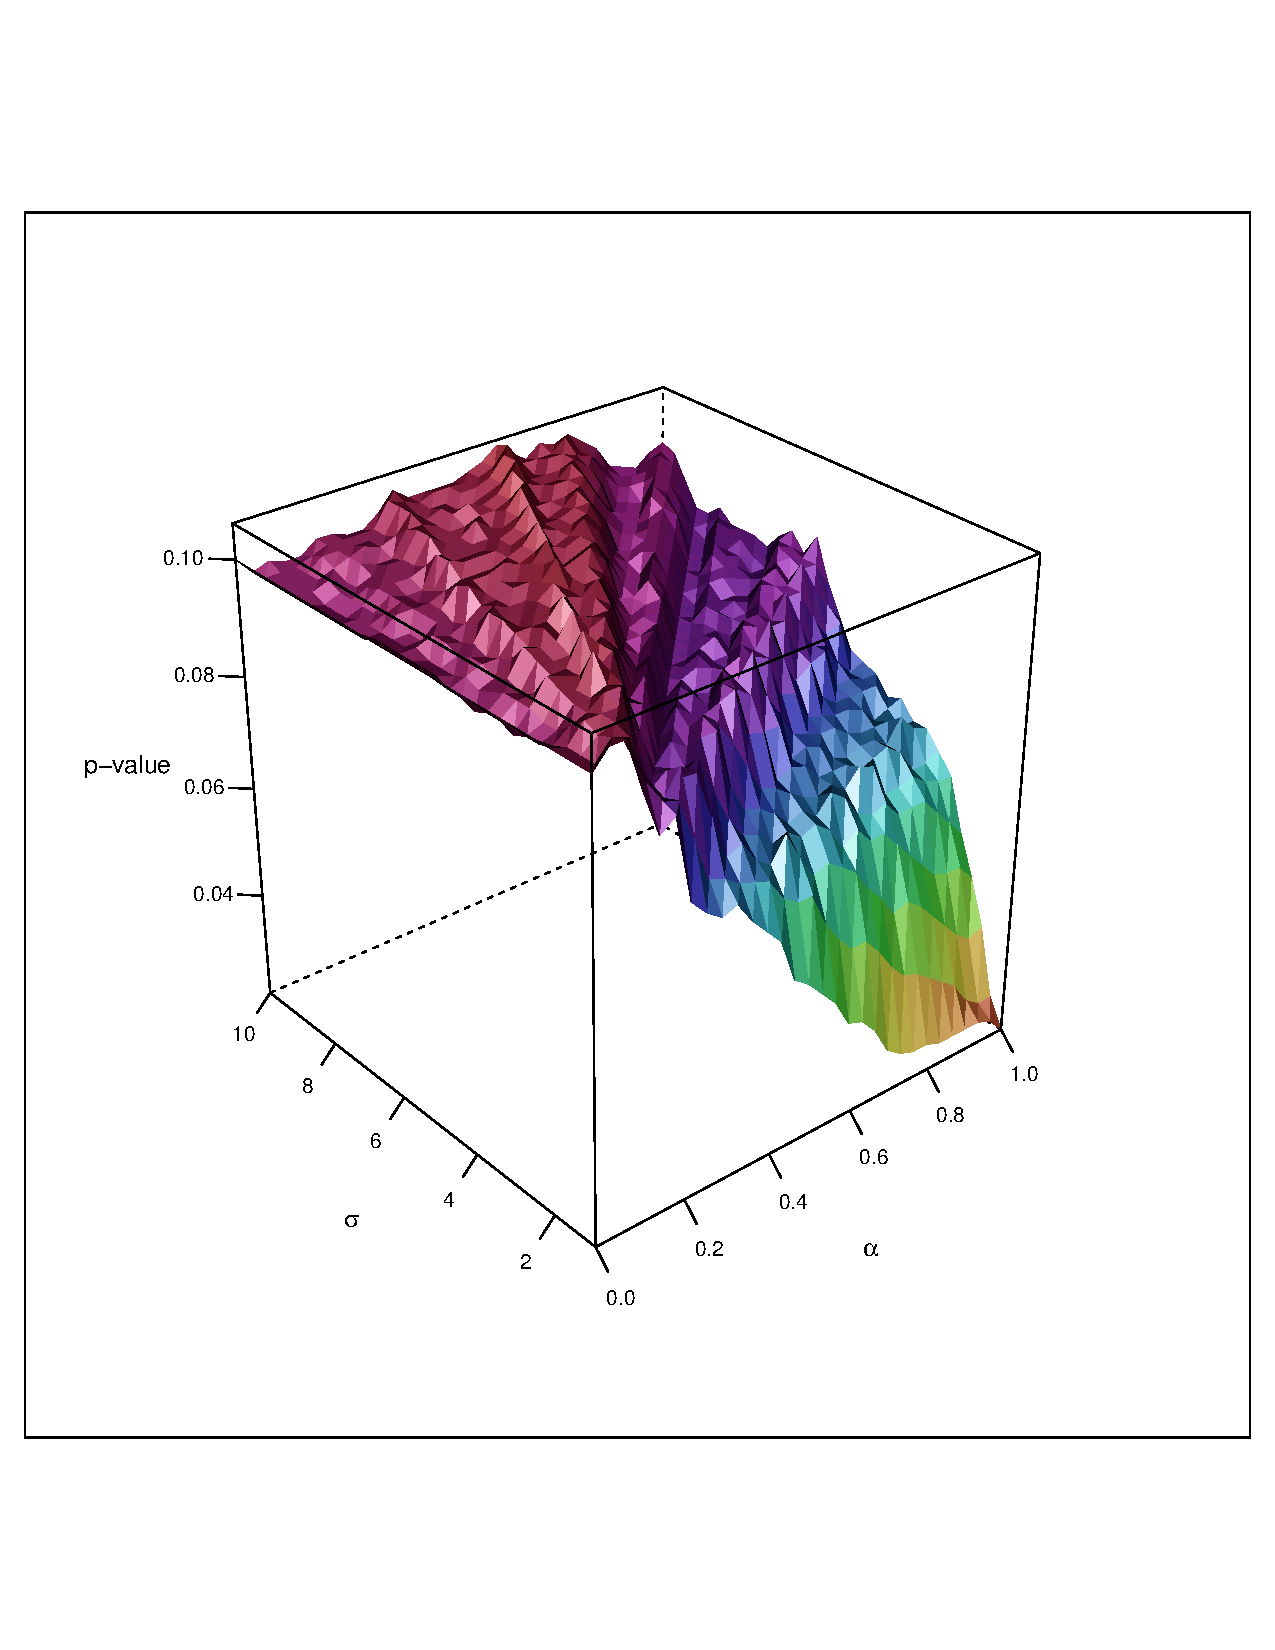
\includegraphics[width=0.7\linewidth]{fig/c-drift}
	\caption{}
	\label{fig:c-drift}
\end{figure}

It is then clear that the ratio of $\frac{\alpha}{\sigma}$ has an influence on the actual distribution of the statistic $t_\gamma$. For $\sigma=1$, as $\alpha$ increases, the simulated p-value decreases. But, as $\sigma$ increases, the effect disappears and the p-value approaches 10\% for any $\alpha$. This points to the fact that the tables given by \cite{fuller_introduction_1976} might not be applicable in case where $\sigma$ is significantly small.

Since, the MMC is robust to this type of problem we get an appropriate level of rejection.

We can extend this problem to the following model
\begin{align}
	Y_t & = \beta t + \frac{1}{2}Y_{t-1} + \frac{1}{2}Y_{t-2} + u_t \quad t = p + 1, ... , T
\end{align}
where $u_t \sim N(0,\sigma^2)$ and $n=25$. Then in figure \ref{fig:ct-trend}, we set the Monte Carlo replications to $N=999$ and we use 10\% asymptotic critical values of the $ct$ model.

\begin{figure}[H]
	\centering
	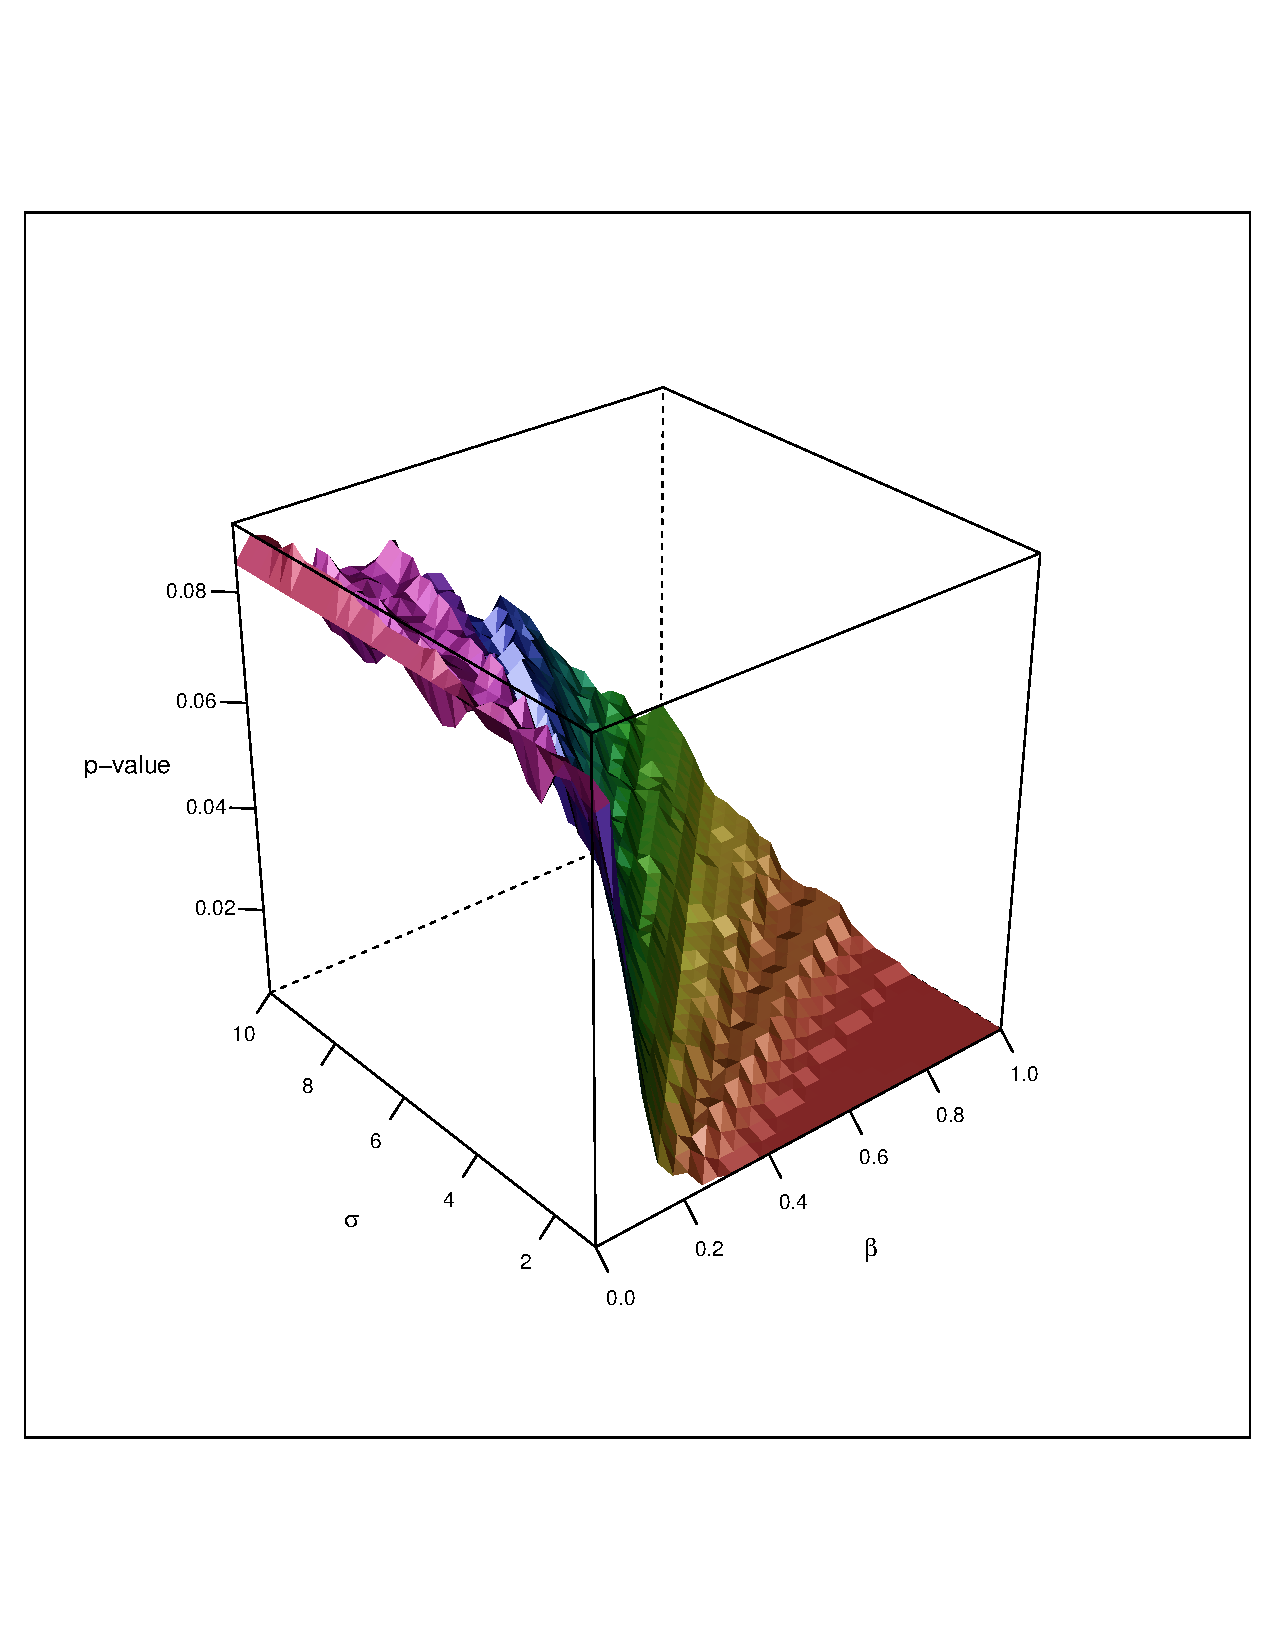
\includegraphics[width=0.7\linewidth]{fig/ct-trend}
	\caption{}
	\label{fig:ct-trend}
\end{figure}

As we can see in figure \ref{fig:ct-trend}, we get the same results as in figure \ref{fig:c-drift}. In fact, the effect is exacerbated by $\beta$ explaining why the bootstrap and the LMC over-reject even more when the model used is $ct$.

Now, in table \ref{tbl:AR:2} and table \ref{tbl:AR:3}, we give the results for $H_1: \gamma > 0$ and $H_1 : \gamma \neq 0$.


\begin{table}[H]
	\centering
	\scalebox{0.8}{
		\begin{tabular}{|r|r|r|r|r|r|r|r|r|r|r|r|r|}
			\hline
			& \multicolumn{4}{|c|}{n = 25} & \multicolumn{4}{|c|}{n = 50} & \multicolumn{4}{|c|}{n = 500}  \\ \hline
			Size & Asy &  Boot & LMC  & MMC & Asy & Boot & LMC & MMC & Asy & Boot & LMC & MMC  \\
			\hline
			nc & 12.4 & 8.8 & 9.6 & 2.8 & 10.8 & 6.8 & 5.6 & 0.8 & 12.0 & 6.0 & 8.4 & 2.0 \\
			c & 50.0 & 11.2 & 13.2 & 2.8 & 40.0 & 11.2 & 10.8 & 1.2 & 39.6 & 4.8 & 5.6 & 0.8 \\
			ct & 32.8 & 5.2 & 6.0 & 0.0 & 28.0 & 6.8 & 6.4 & 0.0 & 26.0 & 2.8 & 3.2 & 0.0 \\
			\hline
		\end{tabular}
	}
	\caption{Empirical levels for 250 replications of I(2) process where $\alpha = 5\%$, testing $H_0: \gamma = 0$ against $H_1:  \gamma > 0$}
	\label{tbl:AR:2}
\end{table}


\begin{table}[H]
	\centering
	\scalebox{0.8}{
		\begin{tabular}{|r|r|r|r|r|r|r|r|r|r|r|r|r|}
			\hline
			& \multicolumn{4}{|c|}{n = 25} & \multicolumn{4}{|c|}{n = 50} & \multicolumn{4}{|c|}{n = 500}  \\ \hline
			Size & Asy &  Boot & LMC  & MMC & Asy & Boot & LMC & MMC & Asy & Boot & LMC & MMC  \\
			\hline
			nc & 10.0 & 11.2 & 7.6 & 3.2 & 8.0 & 7.2 & 4.8 & 1.6 & 11.6 & 9.6 & 7.2 & 4.8 \\
			c & 44.8 & 21.2 & 14.0 & 1.2 & 37.6 & 22.0 & 16.4 & 2.0 & 33.6 & 18.4 & 16.4 & 1.2 \\
			ct & 27.2 & 31.2 & 25.6 & 4.0 & 24.8 & 33.2 & 26.4 & 2.4 & 25.2 & 35.2 & 29.6 & 4.0 \\
			\hline
		\end{tabular}
	}
	\caption{I(2) process, testing $H_0: \gamma = 0$ against $H_1:  \gamma \neq 0$}
	\label{tbl:AR:3}
\end{table}


As predicted by \cite{haldrup_robustness_2002}, the asymptotic test severely over-rejects when $H_1: \gamma>0$. The empirical levels range from 10.8\% up to 50\% for a test with a nominal level of 5\%. This seems to indicate that tests of unit roots such as the augmented Dickey-Fuller might incorrectly classify an I(2) process as an explosive process. In turn, the bootstrap and the LMC seem to perform a bit better than the asymptotic test in this case. The MMC again always under-rejects compared to the 5\% nominal level.

We now consider the three different I(2) models
\begin{align}
	(1-L)^2Y_t = u_t, \quad t=1,...,T \\
	(1-L)(1+L)Y_t = u_t, \quad t=1,...,T \\
	(1-L)^2(1-2L)Y_t = u_t, \quad t=1,...,T
\end{align}
where the $u_t \sim N(0,1)$ are $i.i.d.$

The results are reported in tables \ref{tbl:AR:4}, \ref{tbl:AR:5}  and \ref{tbl:AR:6}.


\begin{table}[H]
	\centering
	\scalebox{0.8}{
		\begin{tabular}{|r|r|r|r|r|r|r|r|r|r|r|r|r|}
			\hline
			& \multicolumn{4}{|c|}{$(1-L)^2 y_t = u_t$} & \multicolumn{4}{|c|}{$(1-L)(1+L) y_t = u_t$} & \multicolumn{4}{|c|}{ $(1-L)^2(1-2L) y_t = u_t$} \\ \hline
			Size & Asy &  Boot & LMC  & MMC & Asy & Boot & LMC & MMC & Asy &  Boot & LMC & MMC  \\
			\hline
			nc & 7.2 & 6.8 & 6.4 & 2.0 & 3.2 & 5.6 & 4.8 & 3.6 & 5.2 & 5.2 & 5.2 & 1.6 \\
			c & 6.4 & 18.0 & 15.2 & 4.0 & 5.2 & 20.4 & 15.6 & 2.8 & 5.6 & 17.2 & 18.0 & 2.8 \\
			ct & 5.6 & 38.0 & 33.2 & 3.2 & 4.0 & 16.4 & 12.4 & 2.4 & 9.6 & 36.8 & 36.0 & 5.6 \\
			\hline
		\end{tabular}
	}
	\caption{Empirical levels for 250 replications of I(2) process where $\alpha = 5\%$ and n=50, testing $H_0: \gamma = 0$ against $H_1:  \gamma < 0$}
	\label{tbl:AR:4}
\end{table}


We can see from table \ref{tbl:AR:4} the asymptotic test slightly over-rejects except for the case where the data generating process is $(1-L)(1+L)Y_t=u_t$ where the empirical levels are fairly close to the nominal ones. In the case of the bootstrap and LMC, when the model is well specified both tests are consistent with the asymptotic results. In the case where the model is misspecified, the bootstrap and MMC have empirical levels well over 15\%. Finally, the MMC is still consistent with the level of 5\%. It usually under rejects except in one case where the empirical level is 5.6\%.


\begin{table}[H]
	\centering
	\scalebox{0.8}{
		\begin{tabular}{|r|r|r|r|r|r|r|r|r|r|r|r|r|}
			\hline
			& \multicolumn{4}{|c|}{$(1-L)^2 y_t = u_t$} & \multicolumn{4}{|c|}{$(1-L)(1+L) y_t = u_t$} & \multicolumn{4}{|c|}{ $(1-L)^2(1-2L) y_t = u_t$} \\ \hline
			Size & Asy &  Boot & LMC  & MMC & Asy & Boot & LMC & MMC & Asy &  Boot & LMC & MMC  \\
			\hline
			nc & 10.8 & 6.8 & 5.6 & 0.8 & 4.4 & 2.8 & 3.6 & 3.6 & 11.6 & 8.4 & 9.6 & 0.0 \\
			c & 40.0 & 11.2 & 10.8 & 1.2 & 4.8 & 1.2 & 1.2 & 0.0 & 43.2 & 13.2 & 13.6 & 0.0 \\
			ct & 28.0 & 6.8 & 6.4 & 0.0 & 4.8 & 2.0 & 3.2 & 0.0 & 34.8 & 6.0 & 5.2 & 0.4 \\
			\hline
		\end{tabular}
	}
	\caption{Empirical levels for 250 replications of I(2) process where $\alpha = 5\%$ and n=50, testing $H_0: \gamma = 0$ against $H_1:  \gamma > 0$}
	\label{tbl:AR:5}
\end{table}


\begin{table}[H]
	\centering
	\scalebox{0.8}{
		\begin{tabular}{|r|r|r|r|r|r|r|r|r|r|r|r|r|}
			\hline
			& \multicolumn{4}{|c|}{$(1-L)^2 y_t = u_t$} & \multicolumn{4}{|c|}{$(1-L)(1+L) y_t = u_t$} & \multicolumn{4}{|c|}{ $(1-L)^2(1-2L) y_t = u_t$} \\ \hline
			Size & Asy &  Boot & LMC  & MMC & Asy & Boot & LMC & MMC & Asy &  Boot & LMC & MMC  \\
			\hline
			nc & 10.8 & 6.8 & 5.6 & 0.8 & 4.4 & 2.8 & 3.6 & 3.6 & 11.6 & 8.4 & 9.6 & 0.0 \\
			c & 40.0 & 11.2 & 10.8 & 1.2 & 4.8 & 1.2 & 1.2 & 0.0 & 43.2 & 13.2 & 13.6 & 0.0 \\
			ct & 28.0 & 6.8 & 6.4 & 0.0 & 4.8 & 2.0 & 3.2 & 0.0 & 34.8 & 6.0 & 5.2 & 0.4 \\
			\hline
		\end{tabular}
	}
	\caption{Empirical levels for 250 replications of I(2) process where $\alpha = 5\%$ and n=50, testing $H_0: \gamma = 0$ against $H_1:  \gamma \neq 0$}
	\label{tbl:AR:6}
\end{table}


Interestingly, the augmented Dickey-Fuller critical values do over-reject for $\gamma>0$ except for the case $(1-L)(1+L) Y_t = u_t$ where the rejection values are actually consistent with the 5\% level. Therefore, the sign of roots might not be trivial in terms of classification of the order of integration of the process.


We now relax the assumption that $u_t~N(0,1)$ and let $u_t$ follow the Student's t distribution with different degrees of freedom (e.g. $df=1,2,3$). The results are reported in tables \ref{tbl:AR:7}, \ref{tbl:AR:8}  and \ref{tbl:AR:9}.


\begin{table}[H]
	\centering
	\scalebox{0.8}{
		\begin{tabular}{|r|r|r|r|r|r|r|r|r|r|r|r|r|}
			\hline
			& \multicolumn{4}{|c|}{$(1-L)^2 y_t = u_t \sim t_1$} & \multicolumn{4}{|c|}{$(1-L)^2 y_t = u_t \sim t_2$} & \multicolumn{4}{|c|}{$(1-L)^2 y_t = u_t \sim t_3$} \\ \hline
			Size & Asy &  Boot & LMC  & MMC & Asy & Boot & LMC & MMC & Asy &  Boot & LMC & MMC   \\
			\hline
			nc & 8.0 & 7.2 & 4.8 & 1.6 & 3.2 & 5.2 & 2.4 & 2.4 & 9.2 & 10.0 & 6.0 & 0.4 \\
			c & 37.6 & 22.0 & 16.4 & 2.0 & 4.4 & 15.6 & 11.6 & 1.6 & 39.2 & 24.0 & 19.2 & 1.6 \\
			ct & 24.8 & 33.2 & 26.4 & 2.4 & 3.6 & 11.2 & 10.0 & 1.6 & 35.2 & 34.4 & 29.2 & 4.4 \\
			\hline
		\end{tabular}
	}
	\caption{Empirical levels for 250 replications of I(2) process where $\alpha = 5\%$ and n=50, testing $H_0: \gamma = 0$ against $H_1:  \gamma < 0$}
	\label{tbl:AR:7}
\end{table}


\begin{table}[H]
	\centering
	\scalebox{0.8}{
		\begin{tabular}{|r|r|r|r|r|r|r|r|r|r|r|r|r|}
			\hline
			& \multicolumn{4}{|c|}{$(1-L)^2 y_t = u_t \sim t_1$} & \multicolumn{4}{|c|}{$(1-L)^2 y_t = u_t \sim t_2$} & \multicolumn{4}{|c|}{$(1-L)^2 y_t = u_t \sim t_3$} \\ \hline
			Size & Asy &  Boot & LMC  & MMC & Asy & Boot & LMC & MMC & Asy &  Boot & LMC & MMC   \\
			\hline
			nc & 11.6 & 7.2 & 7.6 & 2.8 & 12.4 & 8.4 & 9.2 & 2.4 & 15.2 & 8.4 & 9.6 & 3.6 \\
			c & 38.0 & 8.0 & 7.2 & 0.8 & 35.6 & 12.0 & 12.8 & 2.8 & 35.2 & 10.0 & 10.4 & 2.0 \\
			ct & 23.6 & 2.0 & 3.2 & 0.4 & 26.0 & 4.8 & 4.8 & 0.0 & 24.4 & 3.2 & 4.4 & 0.8 \\
			\hline
		\end{tabular}
	}
	\caption{I(2) process with n=50, testing $H_0: \gamma = 0$ against $H_1:  \gamma > 0$}
	\label{tbl:AR:8}
\end{table}


\begin{table}[H]
	\centering
	\scalebox{0.8}{
		\begin{tabular}{|r|r|r|r|r|r|r|r|r|r|r|r|r|}
			\hline
			& \multicolumn{4}{|c|}{$(1-L)^2 y_t = u_t \sim t_1$} & \multicolumn{4}{|c|}{$(1-L)^2 y_t = u_t \sim t_2$} & \multicolumn{4}{|c|}{$(1-L)^2 y_t = u_t \sim t_3$} \\ \hline
			Size & Asy &  Boot & LMC  & MMC & Asy & Boot & LMC & MMC & Asy &  Boot & LMC & MMC   \\
			\hline
			nc & 7.2 & 8.0 & 4.0 & 1.6 & 8.8 & 10.0 & 5.2 & 1.2 & 9.6 & 8.4 & 6 & 1.6 \\
			c & 34.8 & 22.8 & 14.4 & 2.4 & 33.6 & 20.4 & 16.4 & 0.8 & 32.8 & 21.2 & 16 & 2.0 \\
			ct & 22.8 & 30.4 & 25.2 & 3.2 & 23.6 & 34.4 & 27.2 & 3.6 & 24.8 & 34.8 & 26 & 4.8 \\
			\hline
		\end{tabular}
	}
	\caption{Empirical levels for 250 replications of I(2) process where $\alpha = 5\%$ and n=50, testing $H_0: \gamma = 0$ against $H_1:  \gamma \neq 0$}
	\label{tbl:AR:9}
\end{table}


The results of tables \ref{tbl:AR:7}, \ref{tbl:AR:8}  and \ref{tbl:AR:9} are consistent with results when $u_t \sim N(0,1)$. We have over-rejection for every test, except for the MMC.

Finally, we change the order of integration of the process by simulating an I(1) process with increasing order $p$. The results are reported in tables \ref{tbl:AR:10}, \ref{tbl:AR:11}  and \ref{tbl:AR:12}


\begin{table}[H]
	\centering
	\scalebox{0.8}{
		\begin{tabular}{|r|r|r|r|r|r|r|r|r|r|r|r|r|}
			\hline
			& \multicolumn{4}{|c|}{$y_t = \frac{1}{2}\sum_{j=1}^{2}y_{t-j} +u_t$} & \multicolumn{4}{|c|}{$y_t = \frac{1}{3}\sum_{j=1}^{3}y_{t-j} +u_t$} & \multicolumn{4}{|c|}{ $y_t = \frac{1}{4}\sum_{j=1}^{4}y_{t-j} +u_t$} \\ \hline
			Size & Asy &  Boot & LMC  & MMC & Asy & Boot & LMC & MMC & Asy &  Boot & LMC & MMC   \\
			\hline
			nc & 4.0 & 5.6 & 4.8 & 4.8 & 4.4 & 4.0 & 3.2 & 2.0 & 4.8 & 6.4 & 4.8 & 3.2 \\
			c & 3.6 & 19.2 & 15.6 & 1.6 & 4.4 & 20.8 & 17.2 & 2.0 & 2.4 & 18.8 & 18.8 & 0.4 \\
			ct & 5.2 & 18.8 & 17.2 & 2.4 & 3.2 & 19.2 & 17.2 & 0.8 & 2.0 & 20.0 & 17.2 & 2.0 \\
			\hline
		\end{tabular}
	}
	\caption{Empirical levels for 250 replications of I(1) process where $\alpha = 5\%$ and n=50, testing $H_0: \gamma = 0$ against $H_1:  \gamma < 0$}
	\label{tbl:AR:10}
\end{table}


\begin{table}[H]
	\centering
	\scalebox{0.8}{
		\begin{tabular}{|r|r|r|r|r|r|r|r|r|r|r|r|r|}
			\hline
			& \multicolumn{4}{|c|}{$y_t = \frac{1}{2}\sum_{j=1}^{2}y_{t-j} +u_t$} & \multicolumn{4}{|c|}{$y_t = \frac{1}{3}\sum_{j=1}^{3}y_{t-j} +u_t$} & \multicolumn{4}{|c|}{ $y_t = \frac{1}{4}\sum_{j=1}^{4}y_{t-j} +u_t$} \\ \hline
			Size & Asy &  Boot & LMC  & MMC & Asy & Boot & LMC & MMC & Asy &  Boot & LMC & MMC   \\
			\hline
			nc & 4.4 & 5.2 & 4.4 & 4 & 4.8 & 7.2 & 6.4 & 4.8 & 5.2 & 5.6 & 4.4 & 2.0 \\
			c & 3.6 & 1.2 & 1.2 & 0 & 5.6 & 1.6 & 1.6 & 0.4 & 9.2 & 4.8 & 4.4 & 0.4 \\
			ct & 6.8 & 1.6 & 2.0 & 0 & 5.6 & 1.2 & 0.8 & 0.0 & 5.6 & 0.8 & 2.0 & 0.0 \\
			\hline
		\end{tabular}
	}
	\caption{Empirical levels for 250 replications of I(1) process where $\alpha = 5\%$ and n=50, testing $H_0: \gamma = 0$ against $H_1:  \gamma > 0$}
	\label{tbl:AR:11}
\end{table}


\begin{table}[H]
	\centering
	\scalebox{0.8}{
		\begin{tabular}{|r|r|r|r|r|r|r|r|r|r|r|r|r|}
			\hline
			& \multicolumn{4}{|c|}{$y_t = \frac{1}{2}\sum_{j=1}^{2}y_{t-j} +u_t$} & \multicolumn{4}{|c|}{$y_t = \frac{1}{3}\sum_{j=1}^{3}y_{t-j} +u_t$} & \multicolumn{4}{|c|}{ $y_t = \frac{1}{4}\sum_{j=1}^{4}y_{t-j} +u_t$} \\ \hline
			Size & Asy &  Boot & LMC  & MMC & Asy & Boot & LMC & MMC & Asy &  Boot & LMC & MMC   \\
			\hline
			nc & 6.0 & 6.4 & 3.2 & 2.8 & 4.4 & 6.0 & 4.0 & 2.4 & 4.0 & 8.0 & 5.2 & 1.6 \\
			c & 4.4 & 15.2 & 9.2 & 0.8 & 4.4 & 14.0 & 11.2 & 1.2 & 7.2 & 19.2 & 12.0 & 0.4 \\
			ct & 6.8 & 14.8 & 12.8 & 1.6 & 6.0 & 14.8 & 11.2 & 0.8 & 4.4 & 17.2 & 12.8 & 0.8 \\
			\hline
		\end{tabular}
	}
	\caption{Empirical levels for 250 replications of I(1) process where $\alpha = 5\%$ and n=50, testing $H_0: \gamma = 0$ against $H_1:  \gamma \neq 0$}
	\label{tbl:AR:12}
\end{table}


We see that in this I(1) case, the asymptotic critical values give valid inferences. Additionally, the MMC under-rejects in every case. On the other hand, the bootstrap and the LMC are only consistent when $H_1: \gamma>0$. When $H_1: \gamma < 0$, the bootstrap and the LMC severly over-reject.

Therefore, again, only the MMC is valid in every situation.

\subsubsection{Power}

Now, we turn our attention to the power of the different tests. We look at three different data generating processes:
\begin{enumerate}
	\item $y_t = -0.1 y_{t-1} - 0.1  \Delta y_{t-2} +u_t$
	\item $y_t = -0.1 y_{t-1} + 0.1 \Delta y_{t-2} +u_t$
	\item $y_t = 0.1 y_{t-1} - 0.1  \Delta y_{t-2} +u_t$
\end{enumerate}

The results are described in tables \ref{tbl:AR:13}, \ref{tbl:AR:14}  and \ref{tbl:AR:15}


\begin{table}[H]
	\centering
	\scalebox{0.8}{
		\begin{tabular}{|r|r|r|r|r|r|r|r|r|r|r|r|r|}
			\hline
			& \multicolumn{4}{|c|}{$y_t = -0.1 y_{t-1} - 0.1  \Delta y_{t-2} +u_t$} & \multicolumn{4}{|c|}{$y_t = -0.1 y_{t-1} + 0.1 \Delta y_{t-2} +u_t$} & \multicolumn{4}{|c|}{$y_t = 0.1 y_{t-1} - 0.1  \Delta y_{t-2} +u_t$} \\ \hline
			Size & Asy & Boot & LMC & MMC & Asy &  Boot & LMC & MMC & Asy & Boot & LMC & MMC  \\
			\hline
			nc & 21.2 & 23.2 & 19.6 & 14.0 & 27.6 & 30.8 & 28.8 & 23.6 & 0.4 & 0.4 & 0.0 & 0 \\
			c & 10.4 & 18.0 & 12.8 & 2.8 & 10.8 & 26.0 & 20.8 & 4.0 & 0.0 & 0.4 & 0.4 & 0 \\
			ct & 8.0 & 20.4 & 16.4 & 4.4 & 7.2 & 17.6 & 14.8 & 0.8 & 0.0 & 0.0 & 0.0 & 0 \\
			\hline
		\end{tabular}
	}
	\caption{Empirical levels for 250 replications of AR(p) process where $\alpha = 5\%$ and n=50, testing $H_0: \gamma = 0$ against $H_1:  \gamma < 0$}
	\label{tbl:AR:13}
\end{table}


\begin{table}[H]
	\centering
	\scalebox{0.8}{
		\begin{tabular}{|r|r|r|r|r|r|r|r|r|r|r|r|r|}
			\hline
			& \multicolumn{4}{|c|}{$y_t = -0.1 y_{t-1} - 0.1  \Delta y_{t-2} +u_t$} & \multicolumn{4}{|c|}{$y_t = -0.1 y_{t-1} + 0.1 \Delta y_{t-2} +u_t$} & \multicolumn{4}{|c|}{$y_t = 0.1 y_{t-1} - 0.1  \Delta y_{t-2} +u_t$} \\ \hline
			Size & Asy & Boot & LMC & MMC & Asy &  Boot & LMC & MMC & Asy & Boot & LMC & MMC  \\
			\hline
			nc & 0.0 & 0.0 & 0.0 & 0 & 0.0 & 0 & 0.0 & 0 & 96.0 & 96.0 & 96.0 & 96.0 \\
			c & 0.4 & 0.0 & 0.0 & 0 & 0.8 & 0 & 0.4 & 0 & 97.6 & 96.8 & 97.2 & 94.4 \\
			ct & 2.0 & 0.8 & 0.4 & 0 & 2.0 & 0 & 0.0 & 0 & 92.8 & 88.8 & 88.0 & 88.0 \\
			\hline
		\end{tabular}
	}
	\caption{Empirical levels for 250 replications of AR(p) process where $\alpha = 5\%$ and n=50, testing $H_0: \gamma = 0$ against $H_1:  \gamma > 0$}
	\label{tbl:AR:14}
\end{table}


\begin{table}[H]
	\centering
	\scalebox{0.8}{
		\begin{tabular}{|r|r|r|r|r|r|r|r|r|r|r|r|r|}
			\hline
			& \multicolumn{4}{|c|}{$y_t = -0.1 y_{t-1} - 0.1  \Delta y_{t-2} +u_t$} & \multicolumn{4}{|c|}{$y_t = -0.1 y_{t-1} + 0.1 \Delta y_{t-2} +u_t$} & \multicolumn{4}{|c|}{$y_t = 0.1 y_{t-1} - 0.1  \Delta y_{t-2} +u_t$} \\ \hline
			Size & Asy & Boot & LMC & MMC & Asy &  Boot & LMC & MMC & Asy & Boot & LMC & MMC  \\
			\hline
			nc & 11.2 & 14.8 & 9.2 & 6.0 & 14.0 & 21.2 & 12.8 & 8.8 & 95.6 & 96.0 & 95.6 & 95.6 \\
			c & 5.2 & 14.0 & 8.0 & 1.2 & 6.4 & 14.8 & 14.0 & 1.6 & 97.2 & 96.8 & 96.0 & 93.6 \\
			ct & 6.0 & 14.0 & 9.2 & 2.0 & 4.0 & 10.4 & 6.8 & 0.4 & 92.0 & 88.8 & 88.0 & 84.0 \\
			\hline
		\end{tabular}
	}
	\caption{Empirical levels for 250 replications of AR(p) process where $\alpha = 5\%$ and n=50, testing $H_0: \gamma = 0$ against $H_1:  \gamma \neq 0$}
	\label{tbl:AR:15}
\end{table}


Looking at the results it seems that the loss of power of MMC compared to the other tests is minimized when the test is well specified (i.e. when the model is $nc$). Interestingly, the case where $y_t = 0.1 y_{t-1} - 0.1  \Delta y_{t-2} +u_t$, all tests have really high power.

\section{Conclusion}

In this paper, we demonstrated how the \pkg{MaxMC} package provides an easy way to implement Monte Carlo techniques such as the MC technique with tie-breaker and the MMC. These techniques are widely applicable to a wide set of problems. In fact, we demonstrated that with irregular Wald-type tests and unit root tests, only the MMC provides valid inferences compared to the LMC, the bootstrap and the traditional asymptotic distribution.

Future development of the \pkg{MaxMC} package will provide additional tools such as new techniques for global optimization, in order to offer better performance and more versatility to users. Additionally, future versions of \pkg{MaxMC} might include \proglang{C} code. As for the moment, the package is only coded in pure \proglang{R}. This should decrease the computational load required by the \pkg{MaxMC} package.


\clearpage

\printbibliography
\end{document}
